\documentclass[11pt,letterpaper]{report}
\usepackage[left=3.5cm,right=3.5cm,top=2.5cm,bottom=2.5cm]{geometry}

\usepackage{amsmath,amsfonts,amsthm,amssymb,enumitem,mathtools}
\usepackage{hyperref}
\usepackage[spanish]{babel}
\usepackage{todonotes}
\setenumerate[1]{label=(\alph*)}
\setenumerate[0]{label=\roman*.}
\allowdisplaybreaks
\overfullrule=5mm

\setcounter{secnumdepth}{3}
\setcounter{tocdepth}{3}

\newtheorem{defn}{Definición}[chapter]
\newtheorem{theorem}[defn]{Teorema}
\newtheorem{example}[defn]{Ejemplo}
\newtheorem{exe}[defn]{Ejercicio}
\newtheorem{lemma}[defn]{Lema}
\newtheorem{rem}[defn]{Recordatorio}
\newtheorem*{sol}{Solución}
\newtheorem{obs}[defn]{Observación}

\newcommand\R{\mathbb R}
\newcommand\C{\mathbb C}
\newcommand\Z{\mathbb Z}
\newcommand\N{\mathbb N}
\newcommand\norm[1]{\left\|#1\right\|}
\newcommand\<{\langle}
\renewcommand\>{\rangle}
\renewcommand\phi\varphi
\let\cal\mathcal
\let\ol\overline
\DeclareMathOperator{\erf}{erf}
\DeclareMathOperator{\sgn}{sgn}
\DeclareMathOperator{\csch}{csch}
\title{Ecuaciones diferenciales parciales - Notas de clase}
\author{Jorge Alfredo Álvarez Contreras, Ernesto Camacho Ramírez}

\begin{document}
\maketitle

\tableofcontents
\listoftodos

\chapter{Ecuaciones de Primer Orden}

\begin{defn}
  Una ecuación diferencial parcial (EDP) es una ecuación 
  que involucra derivadas de una o más variables dependientes 
  respecto a más de una variable independiente.
\end{defn}

\begin{example}
  Si $u = u(x,y,z)$ entonces
  \[
  \frac{\partial^2 u}{\partial x^2} + \frac{\partial^2 u}{\partial y^2} + \frac{\partial^2 u}{\partial z^2} = 0,
  \] es una EDP conocida com la ecuación de Laplace.
\end{example}

Los conceptos como orden, linealidad, homogeniedad son
similares a los vistos en ecuaciones diferenciales
ordinarias.

\begin{defn}[Orden]
  Es el orden de la máxima o máximas derivadas que aparezcan
  en la EDP.
\end{defn}

\begin{defn}[Linealidad]
  Se dice que una EDP es lineal si la variable o variables
  son \textit{lineales}, así como \textit{todas} sus
  derivadas.
\end{defn}

\begin{example}
  La siguiente ecuación es una EDP de primer orden en dos
  variables $x,y$:
  \[
    P(x,y) z_x + Q(x,y) z_y + R(x,y) z = S(x,y).
  \] 
\end{example}

\begin{example}
  La siguiente EDP es de segundo orden en $x,y$:
  \[
    A(x,y) z_{xx} + 2B(x,y) z_{xy} + C(x,y) z_{yy} + D(x,y)
    z_x + E(x,y) z_y + F(x,y) z = S(x,y),
  \] en donde $P,Q,R,A,B,C,D,E$ y $F$ son funciones
  continuas en alguna región del plano.
\end{example}

\begin{defn}[Ecuación cuasilineal]
  Uan EDP se dice cuasilineal si ésta es lineal en las
  máximas derivadas que aparecen en la ecuación sin importar
  como son los coeficientes.
\end{defn}

\begin{example}
  De primer orden:
  \[
    P(x,y,z)z_x + Q(x,y,z) z_y = R(x,y,z).
  \] 
  De segundo orden:
  \[
    A(x,y,z,z_x,z_y) z_{xx} + B(x,y,z,z_x,z_y) z_{yy} +
    C(x,y,z,z_x,z_y) z_{xy} = R(x,y,z,z_x,z_y).
  \] 
\end{example}

\begin{defn}[Ecuación casilineal]
  La ecuación se dice casilineal si ésta es cuasilineal y
  los coeficientes dependen solo de las variables
  independientes.
\end{defn}

\begin{example}
  De primer orden:
  \[
    P(x,y)z_x + Q(x,y) z_y = R(x,y,z).
  \] 
  De segundo orden:
  \[
    A(x,y) z_{xx} + B(x,y) z_{yy} +
    C(x,y) z_{xy} = R(x,y,z,z_x,z_y).
  \] 

\end{example}

\begin{defn}[Solución de una EDP]
  Por una solución de una EDP se entiende a una función
  $\phi(x,y)$ tal que al sustituirla en la ED, ésta se
  satisface.
\end{defn}

\begin{exe}
  Determine si la función $\displaystyle \phi(x,y) =
  \frac{1}{3}x^3 + xy^2 + c$, donde $c$ es una constante, es
  solución de la ecuación diferencial
  \[
    \frac{\partial z}{\partial x} + z = x, \quad z = z(x,y).
  \] 

  \begin{sol}
    Sea $z = \phi(x,y) = \frac{1}{3}x^3 + xy^2 + c$,
    entonces $z_x = x^2 + y^2$, sustituyendo en la ecuación
    obtenemos
    \[
    x^2 + y^2 + \frac{1}{3}x^3 + xy^2 \neq x,
    \] por lo tanto $\phi$ no es solución de la ecuación
    diferencial.
  \end{sol}
\end{exe}

\begin{exe}
  Sea $\phi(x,y) = e^{x^2}f(x^2+y^2)$ donde $f$ es
  arbitraria. La ecuación es $y z_x - x z_y = 2xyz$.
  
  \begin{sol}
    Primero calculamos las derivdas parciales
    \begin{align*}
      z_x &= 2x e^{x^2} f(x^2 + y^2) + e^{x^2} f'(x^2
      +y^2)2x\\
      z_y &= e^{x^2} f'(x^2+y^2)2y
    \end{align*} 
    Sustituyendo tenemos
    \begin{align*}
      y\left[2x e^{x^2} f(x^2+y^2) + e^{x^2} f'(x^2+y^2)
      2x\right] - 2xy e^{x^2} f'(x^2+y^2) &= 2xy e^{x^2}
      f(x^2+y^2)\\
      \iff 2xy e^{x^2} f(x^2+y^2) + 2xy e^{x^2} f'(x^2+y^2) - 2xy
      e^{x^2} f'(x^2+y^2) &= 2xy e^{x^2} f(x^2+y^2)\\
      \iff 2xy e^{x^2} f(x^2+y^2) &= 2xy e^{x^2} f(x^2+y^2).
    \end{align*} Por lo tanto $\phi$ sí es solución de la
    ecuación.
  \end{sol}
\end{exe}

\section{Obtención de una ecuación diferencial parcial}

\subsection{Por eliminación de funciones arbitrarias}

Dada una familia $z = \phi(x,y)$ de funciones definidas en
cierto dominio del plano, es posible obtener una ecuación
diferencial eliminando las funciones arbitrarias que
aparezcan en ella.

\begin{example}
  Sean $f(x)$ y $g(y)$ dos funciones diferenciables y sea $z
  = f(x) + g(y)$. Determine la ecuación diferencial
  correspondiente a la familia dada.

  \begin{sol}
    Dado que $f$ y $g$ son arbitrarias, la ecuación
    diferencial debe ser de segundo orden. Si $z = f(x) +
    g(y)$, entonces
     \begin{align*}
       z_x &= f'(x)\\
       z_y &= g'(y)\\
       z_{xx} &= f''(x)\\
       z_{yy} &= g''(y)\\
       z_{xy} &= 0.
    \end{align*} Observamos que $z$ satisface la ecuación
    buscada $z_{xy} = 0$.
  \end{sol}
\end{example}

\begin{example}
  Sea $z = f(x)g(y)$. De nuevo
  \begin{align*}
    z_x &= f'(x)g(y)\\
    z_y &= f(x)g'(y)\\
    z_{xx} &= f''(x)g(y)\\
    z_{yy} &= f(x)g''(y)\\
    z_{xy} &= f'(x)g'(y).
  \end{align*}
  Ahora, $z_x z_y = f'(x)g(y)f(x)g'(y) = z_{xy} z$, por lo
  tanto la ecuación buscada es
  \[
    z_{xy} z - z_x z_y = 0.
  \] 
\end{example}

\begin{example}
  Sea $z = e^{-x} f(x-y)$. La solución será de primer orden.
  Las parciales son
  \begin{align*}
    z_x &= -e^{-x} f(x-y) + e^{-x} f'(x-y)\\
    z_y &= -e^{-x} f'(x-y).
  \end{align*} Sumando tenemos
  \[
    z_x + z_y = -e^{-x} f(x-y) = -z \implies z + z_x + z_y =
    0.
  \] 
\end{example}

\subsection{Caso geométrico}

Podemos obtener una ecuación diferencial correspondiente a
los planos tangentes a una superficie.

\begin{enumerate}
  \item Sea $f$ una función diferenciable en una región del
    plano $xy$, entonces la superficie $\mathbb{S}$ en el
    espacio tiene un plano tangente en el punto $(x_0, y_0,
    z_0)$ dada como
    \[
      f_x(x_0, y_0)(x-x_0) + f_y(x_0,y_0)(y-y_0) - (z - z_0)
      = 0.
    \] 
  \item Si $\mathbb{S}$ está dada por la función en forma
    ímplicita $F(x,y,z) = 0$, entonces la ecuación del plano
    tangente a $\mathbb{S}$ en el punto $(x_0,y_0,z_0)$ es
    \[
      F_x(x_0,y_0,z_0)(x-x_0) + F_y(x_0,y_0,z_0)(y-y_0) +
      F_z(x_0,y_0,z_0)(z-z_0) = 0.
    \] 
  \item Supongamos que $\mathbb{S}$ está dada por la
    ecuación en forma paramétrica $x = f(u,v)$, $y = g(u,v)$ 
    y $z = h(u,v)$, donde $u$ y $v$ son parámetros en donde
    los Jacobianos
    \[
      J_1 = \frac{\partial(g,h)}{\partial(u,v)}, \quad J_2 =
      \frac{\partial(f,h)}{\partial(u,v)}, \quad \text{ y }
      \quad J_3 = \frac{\partial(f,g)}{\partial(u,v)}
    \] no son ceros simultáneamente. Entonces la ecuación
    del plano tangente a $\mathbb{S}$ es
    \[
      J_1 \cdot (x-x_0) + J_2 \cdot (y-y_0) + J_3 \cdot
      (z-z_0) = 0.
    \] 
\end{enumerate}

\begin{rem}
  Los Jacobianos se calculan como
  \[
    \renewcommand\arraystretch{1.5}
    J_1 = \begin{vmatrix}
      \frac{\partial g}{\partial u} & \frac{\partial
      g}{\partial v}\\
        \frac{\partial h}{\partial u} & \frac{\partial
        h}{\partial v}
    \end{vmatrix},
  \] donde $J_1, J_2$, y $J_3$ están evaluados en el punto
  $(u_0,v_0)$ correspondiente a $(x_0,y_0,z_0)$.
\end{rem}

El procedimiento se describe en el siguiente ejemplo.

\begin{example}
  Determine la ED de la familia de todos los planos
  tangentes a la elipsoide $x^2 + 4y^2 + 4z^2 = 4$ no
  perpendiculares al plano $xy$.

  \begin{sol}
    Sea $f(x_0,y_0,z_0)$ un punto en la superficie
    $\mathbb{S}$ con $z_0 \neq 0$. Entonces la ecuación del
    plano tangente es
    \[
      F_x(x_0,y_0,z_0)(x-x_0) + F_y(x_0,y_0,z_0)(y-y_0) +
      F_z(x_0,y_0,z_0)(z-z_0) = 0.
    \] Calculando las derivadas parciales
    \[
    F_x = 2x \quad F_y = 8y \quad F_z = 8z,
    \] evaluando en $(x_0,y_0,z_0)$ y sustituyendo obtenemos
    la ecuación del plano tangente
    \begin{align*}
      2x_0(x-x_0) + 8y(y-y_0) + 8z_0(z-z_0) &= 0\\
      \iff xx_0 - x_0^2 + 4yy_0 - 4y_0^2 + 4zz_0 - 4z_0^2 &=
      0\\
      \iff xx_0 - 4yy_0 + 4zz_0 = x_0^2 + 4y_0^2 +
      4z_0^2.
    \end{align*}
    Derivando la ecuación del plano respecto a $x$ y a $y$ 
    obtenemos
    \begin{align*}
      x_0 + 4z_xz_0 = 0 &\implies x_0 = -4z_x z_0\\
      4y_0 + 4z_yz_0 = 0 &\implies y_0 = -z_y z_0.
    \end{align*} Sustituyendo los valores de $x_0$ y $y_0$ 
    en la ecuación del plano obtenemos
    \begin{align*}
      -4x z_0 z_x - 4yz_0 zy + 4z z_0 &= 16z_x^2 z_0^2 +
      4z_y^2 z_0^2 + 4z_0^2\\
      \implies -xz_x - yz_y + z &= (4z_x^2 + z_y^2 + 1)z_0.
    \end{align*}
    Dado que el punto $P(x_0,y_0,z_0)$ pertenece a la
    superficie $\mathbb{S}$, se sigue que $x_0^2 + 4y_0^2 +
    4z_0^2 = 4$. Sustituyendo el valor de $x_0$ y $y_0$ en la
    restricción anterior podemos despejar a $z_0$:
    \begin{align*}
      16z_x^2z_0^2 + 4z_y^2z_0^2 + 4z_0^2 &= 4\\
      \implies (4z_x^2 + z_y^2 + 1)z_0^2 &= 1\\
      \implies z_0^2 = \frac{1}{4z_x^2 + z_y^2 + 1}.
    \end{align*}
    Finalmente sustituímos el valor de $z_0$ en la ecuación
    del plano
    \begin{align*}
      z - xz_x - yz_y &= (4z_x^2 + z_y^2 + 1)
      \frac{1}{(4z_x^2+z_y^2+1)^{1 / 2}}\\
      \implies z - x z_x - y z_ y &= (4z_x^2 + z_y^2 + 1)^{1
      / 2},
    \end{align*}
    o equivalentemente 
    \[
      (z-xz_x - yz_y)^2 = 4z_x^2 + z_y^2 + 1,
    \] la cual es la ecuación diferencial de la familia de
    planos tangentes.

    \begin{figure}[ht]
      \centering
      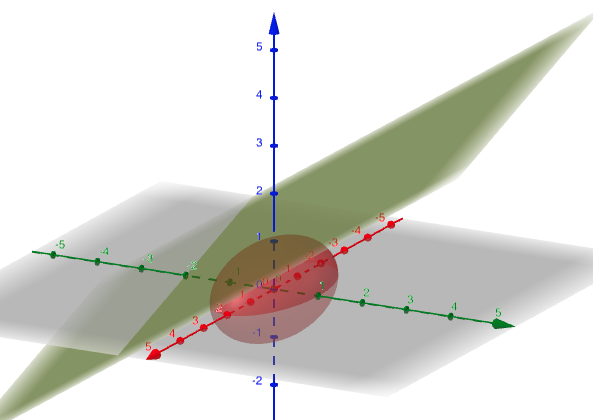
\includegraphics[width=0.5\linewidth]{imgs/chap1-tangent.png}
      \caption{El plano tangente es solución particular de
      la ecuación diferencial anterior.}%
      \label{fig:chap1-tangent}
    \end{figure}
  \end{sol}
\end{example}

\begin{example}
  Determine la ecuación diferencial de la familia de todos los planos tangentes
  a la superficie $\mathbb{S}$ dada por $x^2 - y^2 - z^2 = 0$.

  \begin{sol}
    Sea $P(x_0,y_0,z_0)$ un punto en la superficie $\mathbb{S}$, entonces la
    ecuación del plano tangente es:
    \[
    F_x(x_0,y_0,z_0)(x-x_0) + F_y(x_0,y_0,z_0)(y-y_0) + F_z(x_0,y_0,z_0)(z-z_0)
    = 0,
    \] donde 
    \[
    F_x = 2x, \quad F_y = -2y, \quad F_z = -2z,
    \] evaluando en $(x_0,y_0,z_0)$ obtenemos
    \begin{align*}
      2x_0(x-x_0) - 2y_0(y-y_0) - 2z_0(z-z_0) &= 0\\
      \iff xx_0 - yy_0 - zz_0 = x_0^2 - y_0^2 - z_0^2.
    \end{align*}
    Derivando la ecuación del plano respecto a $x$ y $y$ tenemos
    \begin{align*}
      x_0 - z_x z_0 &= 0 \implies x_0 = z_x z_0\\
      -y_0 - z_y z_0 &= 0 \implies y_0 = -z_y z_0.
    \end{align*}
    Sustituyendo:
    \begin{align*}
      x z_x z_0 + y z_y z_0 - z z_0 &= (z_x z_0)^2 - (z_y z_0)^2 - z_0^2\\
      \iff x z_x + y z_y - z &= (z_x^2 - z_y^2 - 1) z_0.
    \end{align*}
    Como $P \in \mathbb{S}$ y $z_0 \neq 0$, se sigue que
    \begin{align*}
      x_0^2 - y_0^2 - z_0^2 = 0 &\implies (z_x z_0)^2 - (z_y z_0)^2 - z_0^2 =
      0\\
                                &\implies z_x^2 z_0^2 - z_y^2 z_0^2 - z_0^2 =
                                0\\
                                &\implies z_x^2 - z_y^2 - 1 = 0\\
                                &\implies z_x^2 - z_y^2 = 1.
    \end{align*} Así la ecuación diferencial es
    \[
    x z_x + y z_y - z = 0.
    \] 
  \end{sol}
\end{example}

\section{Solución de ecuaciones lineales de primer orden}

Recordemos que una ecuación diferencial lineal es de la
forma
\begin{equation}
  \label{eqn:ed_lineal_1orden}
  A(x,y) z_x + B(x,y) z_y + C(x,y) z = G(x,y),
\end{equation}
donde $A,B,C$ y $G$ son continuas en el plano. La ecuación
más sencilla de resolver es cuando
\ref{eqn:ed_lineal_1orden} contiene solo una derivada
parcial $z_x$ ó $z_y$ ya que se puede manejar como una
ecuación diferencial lineal ordinaria de primer orden:
\[
y' + P(x) y = Q(X),
\] cuya solución es 
\[
y(x) = e^{-\int P(x) \, dx} \left[\int e^{\int P(x) \, dx}
  Q(x) \, dx + C\right].
\] 

\begin{example}
  Resolver $4z_x - 2xz = xy$ donde $z = z(x,y)$.

  \begin{sol}
    Dividiendo por 4 obtenemos $z_x - \frac{1}{2} x z =
    \frac{1}{4} xy$, donde
    \[
    P(x) = -\frac{1}{2} x \quad \text{ y } \quad Q(x) =
    \frac{1}{4} xy.
    \] De acuerdo a lo anterior, la solución está dada por
    \begin{align*}
      z(x,y) &= e^{-\int P(x) \, dx} \left[\int e^{\int P(x)
        \, dx} \, dx + C\right]\\
             &= e^{\frac{1}{2} x \, dx} \left[\int e^{- \int
               \frac{1}{2}x \, dx} \cdot \frac{1}{4} xy \,
               dx + f(y)\right]\\
             &= e^{1 / 4 x^2} \left[-\frac{y}{2} e^{- 1 / 4
               x^2} + f(y)\right]\\
             &= -\frac{y}{2} + e^{1 / 4 x^2} f(y),
    \end{align*}
    donde $f$ es una función arbitraria de $y$.
  \end{sol}
\end{example}

\subsection{Ecuación diferencial homogénea con coeficientes
  constantes}

Consideremos la ecuación
\[
A z_x + B z_y + C z = 0,
\] con $A, B$ y $C$ constantes. Para determinar la solución
de la ecuación se hace el siguiente cambio de variable:
\begin{align*}
  z_x &= z_\xi \xi_x + z_\eta \eta_x = c_{11} z_\xi + c_{21}
  z_\eta\\
  z_y &= z_\xi \xi_y + z_\eta \eta_y = c_{12} z_\xi + c_{22}
  z_\eta.
\end{align*}
Sustituyendo en la ecuación diferencial tenemos
\begin{align*}
  A(z_\xi \xi_x + z_\eta \eta_x) + B(z_\xi \xi_y + z_\eta
  \eta_y) + C z &= 0\\
  \iff A(c_{11} z_\xi + c_{21} z_\eta) + B(c_{12} z_\xi + c_{22}
  z_\eta) + C z &= 0\\
  \iff (A c_{11} + B c_{12}) z_xi + (A c_{21} + B c_{22}) z_\eta
  + C z &= 0,
\end{align*}
donde ahora $z = z(\xi, \eta)$. Ahora, fijemos $c_{11} = 1$,
$c_{12} = 0$, $c_{21} = B$ y $c_{22} = -A$, entonces
la ecuación diferencial anterior se reduce:
\[
A z_\xi + C z = 0,
\] ó equivalentemente (si $A \neq 0$):
\[
z_\xi + \frac{C}{A} z = 0,
\] cuya solución es
\[
z(\xi, \eta) = f(\eta) e^{-\frac{C}{A} \xi}.
\] De acuerdo a la elección de las constantes también
tenemos que
\[
\xi = x, \quad \eta = Bx - Ay,
\] por lo tanto la solución de la ecuación origianl es
\[
z(x,y) = f(Bx - Ay) e^{-\frac{C}{A} x},
\] para $f$ arbitraria.

\begin{obs}
  Para que el cambio de variables sea invertible, es
  necesario que el jacobiano no se anule, en éste caso
  tenemos
  \[
  \frac{\partial(\xi, \eta)}{\partial(x,y)} = -A \neq 0.
  \] 
\end{obs}

\begin{example}
  Resolver la ecuación $3 z_x - 2 z_y + 4z = 0$.
  \begin{sol}
    Notemos que $A = 3$, $B = -2$ y $C = 4$, entonces
    \[
    z(x,y) = f(2x + 3y) e^{-\frac{4}{3} x}.
    \] 
  \end{sol}
\end{example}

\subsection{Ecuación no homogénea}

La ecuación no homogenea es de la forma 
\[
A z_x + B z_y + C z = G(x,y),
\] y recordamos que la solución general de la ecuación no
homogenea es
\[
z = z_h + z_p,
\] donde $z_h$ es la solución a la ecuación homogenea
correspondiente y $z_p$ es una solución particular de la
ecuación no homogenea.

Dicha solución particular se puede determinar mediante el
método de coeficientes indeterminados si $G(x,y)$ es una
combinación de funciones elementales:
\[
\sin, \cos, \exp,
\] con argumentos lineales en $x$ y en $y$, ó cuando $G$ es
un polinomio en $x$ y $y$. 

\begin{example}
  Resolver la ecuación $2 z_x - 3 z_y + z = 5 e^{-2x - y} +
  xy$.
  \begin{sol}
    \begin{enumerate}
      \item Primero obtenemos la solución de la ecuación
        homogenea $2 z_x - 3z_y + z = 0$, la cual está dada
        por
        \[
        z(x,y) = f(3x + 2y) e^{-\frac{1}{2}x}.
        \] 
      \item Ahora obtenemos una solución particular para el
        término $5e^{-2x-y}$. Para ésto proponemos una
        solución de la forma
        \[
        z = A e^{-2x-y},
        \] calculando las derivadas parciales obtenemos
        \[
        z_x = -2 A e^{-2x-y}, \quad z_y = -A e^{-2x-y},
        \] sustituyendo en la ecuación
        \begin{align*}
          2\left(-2Ae^{-2x-y}\right) -
          3\left(-Ae^{-2x-y}\right) + Ae^{-2x-y} &=
          5e^{-2x-y}\\
          \implies -4A + 3A + A &= 5\\
          \implies 0 &= 5,
        \end{align*}
        lo cual es absurdo, por lo tanto la solución
        propuesta no es adecuada, intentemos con $z = A x
        e^{-2x-y}$, entonces
        \[
        z_x = Ae^{-2x-y} - 2Axe^{-2x-y}, \quad z_y =
        -Axe^{-2x-y},
        \] sustituyendo
        \begin{align*}
          2\left(Ae^{-2x-y}-2Axe^{-2x-y}\right) -
          3\left(-Axe^{-2x-y}\right) + Axe^{-2x-y} &=
          5e^{-2x-y}\\
          \implies 2A - 4Ax + 3Ax + Ax &= 5\\
          \implies A = \frac{5}{2},
        \end{align*}
        por lo tanto $z_{p_1} = \frac{5}{2} x e^{-2x-y}$. La
        solución particular $z_{p_2}$ correspondiente al
        término $xy$ se deja como ejercicio para el lector.
    \end{enumerate}
  \end{sol}
\end{example}

\begin{exe}
  Resolver la ecuación de coeficientes constantes no
  homogenea $z_x + 2 z_y = \sin x - 3 \cos y$.
\end{exe}

\begin{example}
  Resolver la ecuación $2z_x + z_y - 2z = \sin(4y-2x)e^{x}$.

  \begin{sol}
    Primero resolvemos la ecuación homogenea correspondiente
    $2z_x + z_y - 2z = 0$. Observemos que $A = 2, B = 1$ y
    $C = -2$, entonces
     \[
      z_h = f(x-2y)e^{x}
    .\] 
    Ahora buscamos una solución particular de la forma
    \[
      z = [A \sin(4y-2x) + B \cos(4y-2x)]e^{x}
    .\] Las derivadas parciales son
    \begin{align*}
      z_x &= [-2A\cos(4y-2x) + 2B\sin(4y-2x)]e^{x} +
      [A\sin(4y-2x) + B\cos(4y-2x)]e^{x}\\
      z_y &= [4A\cos(4y-2x) - 4B\sin(4y-2x)]e^{x}.
    \end{align*}
    Sustituyendo en la ecuación diferencial y simplificando
    obtenemos
    \begin{align*}
      0 &= \sin(4y-2x)e^{x},
    \end{align*}
    lo cual es absurdo, por lo tanto debemos buscar una
    solución particular de otra forma, digamos
    \[
    z = [A\sin(4y-2x) + B\cos(4y-2x)]x e^{x}
    .\] Derivando
    \begin{align*}
      z_x &= [-2A\cos(4y-2x) + 2B\sin(4y-2x)]xe^{x}\\
          &\quad+ [A\sin(4y-2x)+B\cos(4y-2x)](x+1)e^{x}\\
      z_y &= [4A\cos(4y-2x) - 4B\sin(4y-2x)]xe^{x}.
    \end{align*}
    Sustityendo y simplificando obtenemos
    \[
      [2A\sin(4y-2x) + 2B\cos(4y-2x)]e^{x} = \sin(4y-2x)e^{x}
    ,\] 
    por lo tanto $B = 0$ y $A = \frac{1}{2}$, así la
    solución particular es
    \[
    z_p = \frac{1}{2}\sin(4y-2x)xe^{x}
    .\]
    Se sigue que la solución general de la ecuación
    diferencial está dada por
    \[
    z = f(x-2y)e^{x} + \frac{1}{2}\sin(4y-2x)xe^{x}
    .\] 
  \end{sol}
\end{example}

\begin{exe}
  Resolver la ecuación $3z_x - 4z_y + 6z = 4e^{2x+3y}$.
\end{exe}

\subsection{Ecuación homogenea con coeficientes variables}

Consideremos la ecuación la ecuación
\begin{equation}
  \label{eqn:ec_homo_coef_var}
  A(x,y) z_x + B(x,y) z_y + C(x,y) z = 0,
\end{equation} 
con $A,B$ y $C$ funciones continuas en alguna región del
plano. El método para resolver la ecuación
\ref{eqn:ec_homo_coef_var} consiste en encontrar una
transformación $\xi = \xi(x,y)$ y  $\eta = \eta(x,y)$ con
$\frac{\partial(\xi,\eta)}{\partial(x,y)} \neq 0$.

Por la regla de la cadena tenemos
\begin{align*}
  z_x &= z_\xi \xi_x + z_\eta \eta_x\\
  z_y &= z_\xi \xi_y + z_\eta \eta_y,
\end{align*}
sustituyendo en la ecuación
\begin{align*}
  A(z_\xi \xi_x + z_\eta \eta_x) + B(z_\xi \xi_y + z_\eta
  \eta_y) + Cz &= 0\\
  \implies (A\xi_x + B \xi_y)z_\xi + (A\eta_x +
  B\eta_y)z_\eta + Cz &= 0,
\end{align*}
en donde ahora $A,B$ y $C$ son funciones de $\xi, \eta$.
Para simplificar la ecuación anterior, elíjase a $\eta$ de
tal manera que
\[
A\eta_x + B\eta_y = 0,
\] 
es decir
\begin{equation}
  \label{eqn:ec_homo_coef_var_xi_eta}
  \frac{\eta_x}{\eta_y} = -\frac{B}{A}.
\end{equation} 
Ahora suponga que $A \neq 0$ y consideremos la ecuación
diferencial ordinaria
\[
\frac{dy}{dx} = \frac{A}{B},
\] 
cuya solución es $\eta(x,y) = k$ con $\eta_y \neq 0$. Ésta
función satisface \ref{eqn:ec_homo_coef_var_xi_eta}, ya que
\[
\eta_x \, dx + \eta_y \, dy = 0 \implies \frac{dy}{dx} =
-\frac{\eta_x}{\eta_y} = \frac{B}{A}.
\] 
De ésta manera la ecuación queda como
\[
  (A \xi_x + B \xi_y)z_\xi + C z = 0.
\] 
Luego elíjase a $\xi$ como $\xi = x$. Entonces obtenemos la
ecuación diferencial
\[
A z_\xi + C z = 0 \iff z_\xi + \frac{C}{A} z = 0,
\]
cuya solución es
\[
z(\xi,\eta) = f(\eta) e^{-\int \frac{C}{A} \, d\xi}
.\] 
\begin{obs}
  Notemos que la transformación cumple con el requisito:
  \[
  \frac{\partial(\xi,\eta)}{\partial(x,y)} = 
  \begin{vmatrix}
    \xi_x & \xi_y\\
    \eta_x & \eta_y
  \end{vmatrix} = 
  \begin{vmatrix}
    1 & 0\\
    \eta_x & \eta_y
  \end{vmatrix} = \eta_y \neq 0
  .\] 
\end{obs}

\begin{example}
  Resolver la ecuación $xy z_x - x^2 z_y - yz = 0$.
  \begin{sol}
    Los coeficientes de la ecuación están dadas por las
    funciones continuas
    \[
    A = xy, \quad B = -x^2, \quad C = -y.
    \] 
    Observemos que
    \[
    \frac{dy}{dx} = -\frac{x^2}{xy} = -\frac{x}{y},
    \] 
    equivalentemente
    \[
    y \, dy + x \, dx = 0.
    \] 
    La solución de la ecuación anterior es $x^2 + y^2 = k$,
    por lo tanto definamos la transformación $\eta = x^2 +
    y^2$ y $\xi = x$. Aplicando la transformación la
    ecuación se convierte en
    \[
    z_\xi + \frac{C}{A} z = 0 \iff z_\xi - \frac{1}{\xi} z =
    0.
    \]
    Cuya solución es
    \begin{align*}
      z(\xi,\eta) &= f(\eta)e^{-\int -\frac{1}{\xi} \,
      d\xi}\\
                  &= f(\eta)e^{\ln \xi}\\
                  &= \xi f(\eta).
    \end{align*} 
    Expresamos la solución en términos de $x,y$: 
    \[
      z(x,y) = xf(x^2+y^2).
    \] 
  \end{sol}
\end{example}

\begin{example}
  Resolver la ecuación $x^2 z_x - xy z_y + yz = 0.$
  \begin{sol}
    Los coeficientes son las funciones continuas
    \[
    A = x^2, \quad B = -xy, \quad C = y.
    \] 
    Entonces
    \[
    \frac{dy}{dx} = -\frac{xy}{x^2} = -\frac{y}{x} \iff
    \frac{dy}{y} + \frac{dx}{x} = 0,
    \] 
    cuya solución es
    \[
    \ln y + \ln x = \ln k \iff xy = k.
    \]
    Definamos la transformación $\xi = x$ y $\eta = xy$.
    Dado que $\frac{C}{A} = \frac{y}{x^2} =
    \frac{\eta}{\xi^3}$ la ecuación transformada tiene como
    solución
    \[
    z(\xi,\eta) = f(\eta)e^{-\int \frac{\eta}{\xi^3} \, d\xi} =
    f(\eta)e^{\frac{\eta}{2\xi^2}}.
    \] 
    En términos de $x$ y $y$ tenemos
    \[
    z(x,y) = f(xy)e^{\frac{y}{2x}}.
    \] 
  \end{sol}
\end{example}

\begin{example}
  Resolver la ecuación $2x z_x - 3y z_y + 6z = 0$.
  \begin{sol}
    Los coeficientes son las funciones continuas
    \[
    A = 2x, \quad B = -3y, \quad C = 6.
    \] 
    Entonces
    \[
    \frac{dy}{dx} = -\frac{3y}{2x} \implies \frac{dy}{3y} +
    \frac{dx}{2x} = 0,
    \]
    por lo tanto
    \[
    \frac{1}{3}\ln(y) + \frac{1}{2}\ln(x) = \ln k \iff
    x^3y^2 = k.
    \] 
    Sean $\eta = x^3 y^2$ y $\xi = x$. Entonces $\frac{C}{A}
    = \frac{6}{2x} = \frac{3}{\xi}$. Por lo tanto la
    solución de la ecuación transformada es
    \[
    z(x,y) = f(\eta)e^{-\int \frac{3}{\xi} \, d\xi} =
    f(\eta)e^{-3\ln \xi} = f(\eta) \xi^{-3}.
    \] 
    En términos de $x$ y $y$:
    \[
    z(x,y) = \frac{f(x^3y^2)}{x^3}.
    \] 
  \end{sol}
\end{example}

Un caso particular es cuando $A(x,y) = ax, B(x,y) = by$ y
$C(x,y) = c$. La sustitución $\xi = \ln x$ y $\eta = \ln
y$ transforma la ecuación diferencial en una ecuación
diferencial con coeficientes constantes en $\xi, \eta$.

\begin{example}
  Resolver la ecuación $2x z_x - 3yz_y + 6z = 0$.
  \begin{sol}
    Sean $\xi = \ln x$ y $\eta = \ln y$. Entonces
    \[
    z_x = z_\xi \xi_x + z_\eta \eta_x = z_\xi \frac{1}{x},
    \quad \text{ y } \quad z_y = \frac{1}{y} z_\eta.
    \] 
    Sustituyendo obtenemos la ecuación de coeficientes
    constantes
    \[
    2z_\xi - 3z_\eta + 6z = 0.
    \] 
    Cuya solución es
    \[
    z(\xi,\eta) = f(3\xi + 2\eta)e^{-3\xi},
    \] 
    ó
    \[
    z(x,y) = f(x^3y^2)x^{-3}.
    \] 
  \end{sol}
\end{example}

\subsubsection{Ecuación no homogenea}

Para resolver la ecuación no homogenea con coeficientes
variables primero resolvemos la ecuación homogenea
correspondiente y luego obtenemos una solución particular.

\begin{example}
  Resolver la ecuación $x z_x + 2y z_y + z = x\cos x$.
  \begin{sol}
    \begin{itemize}
      \item La ecuación homogenea es $xz_x+2yz_y + z=0$. Sea
        $\xi = \ln x$ y $\eta = \ln y$, entonces la ecuación
        transformada es
        \[
          z_\xi + 2z_\eta + z = 0,
        \] 
        cuya solución es
        \[
          z_h = f(2\xi - \eta)e^{-\xi}.
        \] 
        En términos de $x,y$:
        \[
        z_h = f(2\ln x - \ln y)e^{-\ln x} = \frac{1}{x}
        f\left(\frac{x^2}{y}\right).
        \] 
      \item Para obtener la solución particular, observemos
        que $G(x,y) = x \cos x$ solo depende $x$ por lo que
        se puede eliminar el término con $z_y$, es decir, el
        problema se reduce a resolver la ecuación ordinaria
        \[
        x z_x + z = x\cos x.
        \] 
        La solución particular está dada por
        \begin{align*}
          z_p &= e^{-\int \frac{1}{x}\, dx} \left(\int
            e^{\int \frac{1}{x} \, dx} \cos x \, dx +
            g(y)\right)\\
              &= e^{-\int \frac{dx}{x}} \int e^{\int
              \frac{dx}{x}} \cos x \, dx\\
              &= x^{-1} \int x\cos x \, dx\\
              &= x^{-1}\left(x\sin x + \cos x\right)\\
              &= \sin x + \frac{\cos x}{x}.
        \end{align*}
    \end{itemize}
    Se sigue que la solución de la ecuación diferencial es
    \[
    z = \frac{1}{x}f\left(\frac{x^2}{y}\right) + \sin x +
      \frac{1}{x} \cos x.
    \] 
  \end{sol}
\end{example}

\begin{example}
  Resolver $(x+2)z_x - (y-1)z_y + 2z = 2x + 3y$.
  \begin{sol}
    \begin{itemize}
      \item Primero resolver la ecuación homogenea
        correspondiente. Los coeficientes continuos son
        \[
        A = x + 2, \quad B = 1 - y, \quad c = 2.
        \] 
        Entonces
        \[
        \frac{dy}{dx} = -\frac{y-1}{x+2} \implies
        \frac{dy}{y-1} + \frac{dx}{x+2} = 0.
        \] 
        Resolviendo obtenemos
        \[
        \ln(y-1) + \ln(x+2) = \ln(k) \implies (x+2)(y-1) =
        \eta.
        \] 
        Sean $\xi = x$ y $\eta = (x+2)(y-1)$. Se sigue que
        $\frac{C}{A} = \frac{2}{\xi + 2}$. Entonces la
        solución está dada por
        \[
        z(\xi,\eta) = f(\eta)e^{-\int \frac{2}{\xi+2} \,
        d\xi} = f(\eta)(\xi+2)^{-2}.
        \] 
        Expresamos la solución de la ecuación homogenea en
        términos de $x$ y $y$:
        \[
        z_h = f((x+2)(y-1)) \frac{1}{(x+2)^2}.
        \] 
      \item Separemos el término $G(x,y) = 2x + 3y$ en dos.
        Primero sea $G_1(x,y) = 2x$. Por el mismo
        razonamiento buscamos resolver la ecuación 
        \[
          (x+2)z_x + 2z = 2x \iff z_x + \frac{2}{x+2}z =
          \frac{2x}{x+2}.
        \] 
        La solución es
        \begin{align*}
          e^{-\int \frac{2}{x+2} \, dx} \left(\int e^{\int
            \frac{2}{x+2} \, dx} \frac{2x}{x+2} \, dx\right)
            &=
            e^{-2\ln(x+2)}\left(\int e^{2\ln(x+2)}
            \frac{2x}{x+2} \, dx\right)\\
            &=
            \frac{1}{(x+2)^2}\left(\int (x+2)^2
            \frac{2x}{x+2} \, dx\right)\\
            &= \frac{1}{(x+2)^2} \int
            \left(2x^2 + 4x\right) \, dx\\
            z_{p_1} &= \frac{x^2(x+3)}{(x+2)^2}.
        \end{align*}
        La solución correspondiente a $G_2(x,y) = 3y$ y por
        lo tanto la solución general de la ecuación se dejan
        como ejercicio al lector.
    \end{itemize}
  \end{sol}
\end{example}

\section{Solución de la ecuación cuasilineal}

\subsection{Método de Lagrange}

Recordemos que la ecuación cuasilineal de primer orden en
$x$ y $y$ de la forma
\begin{equation}
  \label{eqn:cuasilineal_primer_orden}
  P(x,y,z) z_x + Q(x,y,z) z_y = R(x,y,z),
\end{equation}
donde $P, Q$ y $R$ son funciones con las derivadas parciales
continuas. Por una solución
\ref{eqn:cuasilineal_primer_orden} se entiende a una función
$\phi(x,y)$ con derivadas parciales tales que si $(x_0,y_0)$
es un punto del dominio del plano $xy$ entonces $z_0 =
\phi(x_0,y_0)$ y además
\[
P(x,y,\phi) \phi_x + Q(x,y,\phi) \phi_y = R(x,y,\phi).
\] 
Si $z = \phi(x,y)$ es la solución de
\ref{eqn:cuasilineal_primer_orden}, entonces $z_x, z_y$
deben satisfacer \ref{eqn:cuasilineal_primer_orden}
\begin{equation}
  \label{eqn:derivada_total_cuasi}
  dz = \phi_x \, dx + \phi_y \, dy = z_x \, dx + z_y \, dy.
\end{equation}
Si \ref{eqn:derivada_total_cuasi} representa a
\ref{eqn:cuasilineal_primer_orden}, entonces tenemos que
\begin{align*}
  dx &= KP(x,y,z)\\
  dy &= KQ(x,y,z)\\
  dz &= KR(x,y,z).
\end{align*}
Por lo tanto obtenemos la ecuación
\begin{equation}
  \label{eqn:subsidiaria}
  \frac{dx}{P} = \frac{dy}{Q} = \frac{dz}{R},
\end{equation}
la cual es llamada \textit{ecuación subsidiaria} ó
\textit{ecuación característica} de
\ref{eqn:cuasilineal_primer_orden}. De \ref{eqn:subsidiaria}
se obtienen dos ecuaciones diferenciales ordinarias:
\[
\frac{dx}{P} = \frac{dy}{Q} \quad \text{ y } \quad
\frac{dx}{P} = \frac{dz}{R}.
\] 
Podemos suponer que la variable independiente es $x$. Sean
$y = y(x,c_1,c_2)$ y
$z = z(x,c_1,c_2)$ las soluciones, donde
$c_1$ y $c_2$ son constantes arbitrarias. Si éstas
ecuaciones son resueltas para $c_1$ y $c_2$ se obtiene
\[
c_1 = u(x,y,z) \quad \text{ y } \quad c_2 = v(x,y,z).
\] 
Éstas son llamadas \textit{curvas integrales} de la ecuación
subsidiaria. De ésta forma la relación $F(c_1,c_2) = 0$ es
la solución
de \ref{eqn:cuasilineal_primer_orden}, es decir
\[
F(u(x,y,z), v(x,y,z))=0.
\] 
\begin{example}
  Resolver la ecuación $xz z_y + yz z_y = -(x^2+y^2)$.
  \begin{sol}
    Los coeficientes son
    \[
    P = xz, \quad Q = yz, \quad R = -(x^2+y^2).
    \] 
    La ecuación subsidaria está dada por
    \[
    \frac{dx}{xz} = \frac{dy}{yz} = \frac{dz}{-x^2-y^2}.
    \] 
    Se sigue que tenemos dos EDO por resolver, elegimos las
    siguientes
    \[
    \frac{dx}{x} = \frac{dy}{y} \quad \text{ y } \quad
    \frac{dx}{zx} = \frac{dz}{-x^2-y^2}.
    \] 
    Resolviendo la primera obtenemos la primera curva
    integral
    \begin{align*}
      \ln x &= \ln y + \ln c_1\\
      \implies x &= yc_1\\
      \implies c_1 &= \frac{x}{y}.
    \end{align*}
    Para la segunda tenemos
    \begin{align*}
      \frac{dx}{xz} &= \frac{dz}{-x^2-y^2}\\
      \implies \frac{dx}{xz} &= \frac{dz}{-x^2-x^\frac{2}{c_1^2}}\\
      \implies -x \, dx &= \frac{z \, dz}{1 + \frac{1}{c_1^2}}\\
      \implies x\left(1+\frac{1}{c_1^2}\right) \, dx + z \, dz &= 0\\
      \implies \left(1+\frac{1}{c_1^2}\right) \frac{x^2}{2} +
      \frac{z^2}{2} &= \frac{c_2}{2}.
    \end{align*}
    Sustituyendo $c_1$ obtenemos la segunda curva integral
    \[
    c_2 = \left(1+\frac{y^2}{x^2}\right) x^2 + z^2 = x^2 +
    y^2 + z^2.
    \] 
    Se sigue que la solución de la ecuación es
    \[
    F(c_1,c_2) = F\left(\frac{x}{y}, x^2+y^2+z^2\right) = 0,
    \] 
    para $F$ arbitraria.
  \end{sol}
\end{example}

\subsection{Método de multiplicadores}

Otra forma de resolver la ecuación subsidiaria es mediante
multiplicadores. Sea $\alpha, \beta, \gamma$ cualesquier
valor, entonces tenemos las siguientes igualdades
\[
\frac{\alpha \, dx + \beta \, dy + \gamma \, dz}{\alpha P +
\beta Q + \gamma R} = \frac{dx}{P} = \frac{dy}{Q} =
\frac{dz}{R}.
\] 
En particular si se elige a $\alpha, \beta, \gamma$ de tal
manera que
\[
\alpha P + \beta Q + \gamma R = 0,
\] 
entonces se tiene que
\[
\alpha \, dx + \beta \, dy + \gamma \, dz = 0.
\] 

\begin{example}
  Resolver la ecuación $(y-x) z_x + (y+x) z_y = (x^2+y^2) /
  z$.
  \begin{sol}
    La ecuación subsidiaria está dada por
    \[
    \frac{dx}{y-x} = \frac{dy}{y+x} = \frac{z \,
    dz}{x^2+y^2}.
    \] 
    Utilizando el método de Lagrange sin multiplicadores
    resultará complicado, en lugar de resolver alguna de las
    ecuaciones definamos $\alpha = x$, $\beta = -y$ y
    $\gamma = z$. Entonces
    \[
    x(y-x) - y(y+x) + z\left(\frac{x^2+y^2}{2}\right) = xy -
    x^2 - y^2 - xy + x^2 + y^2 = 0.
    \]
    Por lo tanto podemos resolver la ecuación
    \[
    x \, dx - y \, dy + z \, dz = 0,
    \] 
    para obtener la primera curva integral
    \[
    x^2 - y^2 + z^2 = c_1.
    \] 
    Ahora, si $\alpha = 1, \beta = 1$ y $\gamma = 0$,
    entonces
    \[
    \frac{dx + dy}{y - x + y + x} = \frac{dy}{x + y},
    \] 
    ó equivalentemente
    \[
      (x+y)(dx + dy) = 2y \, dy.
    \] 
    Integrando obtenemos
    \[
    \frac{(x+y)^2}{2} = y^2 + c \implies c_2 = x^2 + 2xy -
    y^2.
    \] 
    Las curvas son linealmente independientes y así
    obtenemos la solución de la ecuación 
    \[
    F(c_1,c_2) = F\left(x^2 - y^2 +
      z^2, x^2 + 2xy - y^2\right) = 0.
    \] 
  \end{sol}
\end{example}

\begin{obs}
  Si por ejemplo $R = 0$, entonces la ecuación subsidiaria
  es de la forma
  \[
  \frac{dx}{P} = \frac{dy}{Q} \quad \text{ y } \quad dz = 0.
  \] 
\end{obs}

\begin{example}
  Resolver la ecuación $(x+z) z_x + (y+z) z_y = 0$.
  \begin{sol}
    La ecuación subsidiaria es
    \[
    \frac{dx}{x+z} = \frac{dy}{y+z} \quad \text{ y } \quad
    dz = 0.
    \] 
    Se sigue que $z = c_1$ es una curva integral.
    Sustituyendo el valor de $z$ en la primera ecuación,
    obtenemos una ecuación separable
    \[
    \frac{dx}{x+c_1} = \frac{dy}{y+c_1},
    \]
    integrando obtenemos $\ln(x+c_1) = \ln(y+c_1) +
    \ln(c_2)$, es decir
    \[
    c_2 = \frac{x+z}{y+z}.
    \] 
    Se sigue que la solución es
    \[
    F\left(z, \frac{x+z}{y+z}\right) = 0,
    \] 
    para $F$ arbitraria.
  \end{sol}
\end{example}

\begin{example}
  Resolver la ecuación $(3z-4y) z_x + (4x+5z) z_y = -5y -
  3x$.
  \begin{sol}
    La ecuación subsidiaria es
    \[
    \frac{dx}{3z-4y} = \frac{dy}{4x+5z} = \frac{dz}{-5y-3x}.
    \] 
    Sean $\alpha = x, \beta = y$ y $\gamma = z$. Entonces
    \[
    \alpha P + \beta Q + \gamma R = 3xz - 4xy + 4xy + 5yz -
    5yz - 3xz = 0.
    \] Por lo tanto
    \[
    x \, dx + y \, dy + z \, dz = 0 \implies c_1 = x^2 + y^2
    + z^2.
    \] 
    Ahora fijemos $\alpha = -5, \beta = 3$ y $\gamma = 4$,
    entonces
    \[
    -5(3z-4y) + 3(4x+5z) + 4(-5y-3x) = -15z + 20y + 12x +
    15z - 20y - 12x = 0.
    \]
    Se sigue que
    \[
    -4 \, dx + 3 \, dy + 4 \, dz = 0 \implies c_2 = -5x + 3y
    + 4z.
    \] 
    La solución es
    \[
    F\left(x^2+y^2+z^2, -5x + 3y + 4z\right) = 0.
    \] 
  \end{sol}
\end{example}

\section{Problemas de Cauchy de primer orden}

Al igual que un problema de valor inicial para una ecuación
diferencial ordinaria, existen para las ecuaciones
diferenciales parciales los llamados problemas de Cauchy los
cuales consisten en determinar la solución de la ecuación
cuasilineal
\begin{equation}
  \label{eq:cauchy_ec_cuasi}
  P z_x + Q z_y = R.s,
\end{equation}
y que pasa por una curva $\Gamma$ dada por lo general en
forma paramétrica. Es decir, sea $\Gamma$ una curva
\textit{suave} dada por $x = f(t), y = g(t)$ y $z = h(t)$
con $a \leq t \leq b$. Para determinar la superficie
integral de \ref{eq:cauchy_ec_cuasi} que contenga a $\Gamma$
se procede como sigue.

Sean $u(x,y,z) = c_1$ y $v(x,y,z) = c_2$ las curvas
integrales de la ecuación subsidiaria
\[
\frac{dx}{P} = \frac{dy}{Q} = \frac{dz}{R},
\] 
se puede escribir $c_1 = u(x(t), y(t), z(t))$ y $c_2 =
v(x(t),y(t),z(t))$ y eliminando el parametro $t$ obtenemos
la relación entre $c_1$ y $c_2$ tal que $F(u,v,) = 0$ para
alguna función $F$.

\begin{example}
  Resolver la ecuación $(y+xz) z_x + (x+yz) z_y = z^2 - 1$ y
  que contenga la curva $\Gamma$ dada por $x = t, y = 1$ y
  $z = t^2$.
  \begin{sol}
    La ecuación subsidiaria es
    \[
    \frac{dx}{y+xz} = \frac{dy}{x+yz} = \frac{dz}{z^2-1},
    \] 
    utilizando el método de multiplicadores, elejimos
    $\alpha = 1, \beta = 1$ y $\gamma = 0$. Así
    \[
      \frac{dx+dy}{x+y+z(x+y)} = \frac{dx+dy}{(x+y)(z+1)} =
      \frac{dz}{z^2-1},
    \] 
    entonces
    \[
    \frac{dx+dy}{x+y} = \frac{dz}{z-1} \implies \ln(x+y) =
    \ln(z-1) + \ln c_1 \implies c_1 = \frac{x+y}{z-1}.
    \] 
    Ahora sean $\alpha = x, \beta = -y$ y $\gamma = 0$,
    entonces
    \[
    \frac{x \, dx - y \, dy}{xy + x^2z - xy - y^2z} =
    \frac{dz}{z^2-1},
    \] 
    entonces
    \[
    \frac{x \, dx - y \, dy}{x^2-y^2} = \frac{z \,
    dz}{z^2-1} \implies \ln(x^2-y^2) = \ln(z^2-1) + \ln c_2,
    \] 
    es decir
    \[
    c_2 = \frac{x^2-y^2}{z^2-1}.
    \] 
    De lo anterior tenemos que la solución de la ecuación es
    \[
    F\left(\frac{x+y}{z-1}, \frac{x^2-y^2}{z^2-1}\right) =
    0.
    \]
    Para resolver el problema de Cauchy buscamos relacionar
    las curvas integrales $c_1$ y $c_2$. Aplicando $\Gamma$ 
    a $c_1$ y $c_2$ tenemos
    \[
    c_1 = \frac{t+1}{t^2-1} = \frac{1}{t-1} \implies t =
    \frac{1}{c_1} = 1,
    \] 
    y
    \[
    c_2 = \frac{t^2-1}{t^4 - 1} =
    \frac{t^2-1}{(t^2-1)(t^2+1)} = \frac{1}{t^2+1} \implies
    c_2 = \frac{1}{\left(\frac{1}{c_1}+1\right)^2+1}.
    \] 
    Sustituyendo las curvas integrales obtenemos la solución
    al problema de Cauchy:
    \begin{align*}
      c_2 \left[(1+c_1)^2 + c_1^2\right] &= c_1^2\\
      \implies
      \frac{x^2-y^2}{z^2-1}\left[\left(1+\frac{x+y}{z-1}\right)^2
    + \left(\frac{x+y}{z-1}\right)^2 \right] &=
        \left(\frac{x+y}{z-1}\right)^2.
    \end{align*}
  \end{sol}
\end{example}

\begin{example}
  Resolver el problema de Cuachy: $yz z_x + xz z_y + 2xy =
  0$, con $\Gamma : x^2 + y^2 = 16$ y $z = 3$.
  \begin{sol}
    La ecuación subsidiaria es
    \[
    \frac{dx}{yz} = \frac{dy}{xz} = \frac{dz}{-2xy},
    \] 
    resolviendo las ecuaciones
    \[
    \frac{dx}{yz} = \frac{dy}{xz} \implies \frac{dx}{y} =
    \frac{dy}{x} \implies x^2 - y^2 = c_1.
    \]
    y
    \[
    \frac{dx}{yz} = \frac{dz}{-2xy} \implies \frac{dx}{z} =
    \frac{dz}{-2x} \implies 2x^2 + z^2 = c_2,
    \] 
    obtenemos la solución de la ecuación difernecial
    \[
    F(x^2 - y^2, 2x^2 + z^2) = 0.
    \] 
    Equivalentemente, podemos escribir la solución de la
    siguiente manera
    \[
    c_2 = f(c_1) \implies z^2 = f(x^2-y^2) - 2x^2.
    \] 
    Aplicando $\Gamma$ tenemos
    \[
    f(x^2 - 16 + x^2) = 2x^2 + 9 \iff f(2x^2 - 16) = 2x^2 +
    9.
    \]
    Sea $u = 2x^2 - 16$ entonces
    \[
    2x^2 = u + 16 \implies f(u) = u + 25,
    \] 
    y hemos econtrado a $f$, ahora si $u = x^2 - y^2$
    entonces
    \[
    f(x^2-y^2) = x^2-y^2 + 25 = 2x^2 + z^2 \implies x^2 +
    y^2 + z^2 = 25,
    \] 
    es la solución al problema de Cauchy, ver figura
    \ref{fig:cauchy-esfera-ejemplo}.
    \begin{figure}[ht]
      \centering
      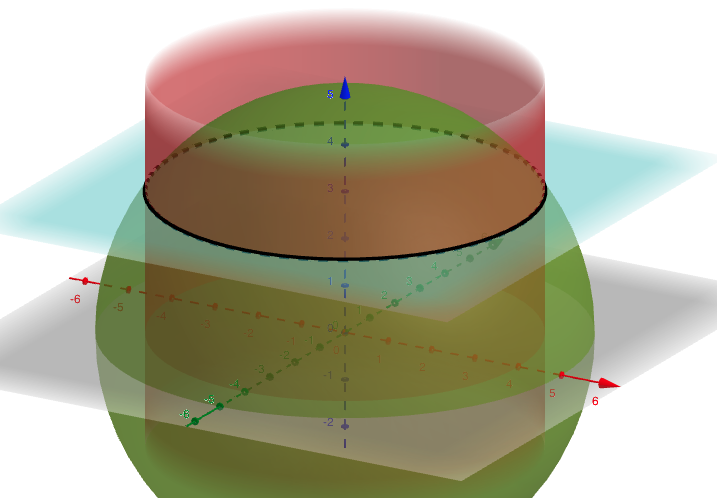
\includegraphics[width=0.6\textwidth]{imgs/cauchy-esfera.png}
      \caption{La esfera es la solución de la ecuación
      diferencial que contiene a la curva $\Gamma$.}
      \label{fig:cauchy-esfera-ejemplo}
    \end{figure}
  \end{sol}
\end{example}

\begin{example}
  Resolver el problema de Cauchy dado por la ecuación
  $(y-z)z_x + (z-x)z_y = x-y$ y la curva $\Gamma : x = t, y
  = 2t, z = 0$.
  \begin{sol}
    La ecuación subsidiaria es
    \[
    \frac{dx}{y-z} = \frac{dy}{z-x} = \frac{dz}{x-y}.
    \] 
    Observemos que $dx + dy + dz = 0 \implies x + y + z =
    c_1$. Similarmente obtenemos la segunda curva integral
    dada por $c_2 = x^2 + y^2 + z^2$. Aplicando $\Gamma$ 
    tenemos que $t + 2t = c_1$ y $t^2 + 4t^2 = c_2$, es
    decir
    \[
    3t = c_1 \implies t = \frac{c_1}{3} \implies
    \frac{5}{9}c_1^2 = c_2.
    \] 
    Sustituyendo las curvas integrales obtenemos la
    solución del problema de Cauchy:
    \[
    5(x+y+z)^2 = 9(x^2+y^2+z^2).
    \] 
  \end{sol}
\end{example}

\begin{example}
  Resolver el problema de Cauchy dado por $(x^2+y^2) z_x +
  2xy z_y = xz$ y $\Gamma : y^2 + z^2 = 4, x = 2$.
  \begin{sol}
    La ecuación subsidiaria es
    \[
    \frac{dx}{x^2+y^2} = \frac{dy}{2xy} = \frac{dz}{xz},
    \] 
    cuyas curvas integrales están dadas por
    \[
    c_1 = \frac{y}{z^2} \quad \text{ y } \quad c_2 =
    \frac{x^2-y^2}{y}.
    \] 
    La solución de la ecuación diferencial está dada por
    \[
    c_2 = f(c_1) \implies \frac{y}{z^2} =
    f\left(\frac{x^2-y^2}{y}\right).
    \] 
    Aplicando $\Gamma$ obtenemos
    \[
    \frac{y}{4-y^2} = f\left(\frac{4-y^2}{y}\right) \implies
    f(u) = \frac{1}{u},
    \] 
    donde $u = \frac{4-y^2}{y}$. Se sigue que
    \[
    \frac{y}{z^2} = \frac{y}{x^2-y^2} \implies \frac{1}{z^2}
    = \frac{1}{x^2-y^2},
    \] 
    por lo tanto la superficie que es solución de la
    ecuación diferencial y contiene a la curva $\Gamma$ está
    dada por
    \[
    x^2 - y^2 - z^2 = 0.
    \] 
  \end{sol}
\end{example}

\chapter{Ecuaciones de Segundo Orden}

\section{Ecuaciones diferenciales parciales de segundo orden
  en dos variables}

Recordemos que la ecuación diferencial lineal de segundo
orden es de la forma
\begin{equation}
  \label{eq:ec_lineal_seg_orden}
  A(x,y) z_{xx} + 2B(x,y)z_{xy} + C(x,y) z_{yy} + D(x,y) z_x
  + E(x,y) z_y + F(x,y) z = G(x,y).
\end{equation}a
donde $A,B,C,D,E,F$ y $G$ son continuas en alguna región del
plano $xy$. Para simplificar \ref{eq:ec_lineal_seg_orden}
introducimos el operador lineal $D$ haciendo
\[
\frac{\partial}{\partial x} = D_x, \quad
\frac{\partial^2}{\partial x^2} = D_{xx} = D_x^2, \quad
\frac{\partial}{\partial x \partial y} = D_{xy} = D_x D_y.
\] 
Así tenemos
\[
  (AD_x^2 + 2BD_xD_y + CD_y^2 + DD_x + ED_y + F)z = G.
\] 
Definamos $L := AD_x^2 + 2BD_xD_y + CD_y^2 + D D_x + ED_y =
F$, entonces la ecuación diferencial se expresa como
\begin{equation}
  \label{eq:ec_expr_diferencial}
  Lz = G(x,y).
\end{equation}
A $L$ se le llama operador diferencial correspondiente a la
ecuación \ref{eq:ec_lineal_seg_orden}. Éste operador es
lineal ya que
\[
L(c_1z_1 + c_2z_2) = c_1 Lz_1 + c_2 Lz_2,
\] 
donde $c_1$ y $c_2$ son constantes y $z_1 = z_1(x,y)$ y
$z_2 = z_2(x,y)$ son funciones diferenciables.

A partir de la linealidad de $L$ se tiene que si
$z_1,z_2,\ldots,z_k$ son soluciones de la ecuación homogenea
\begin{equation}
  \label{eq:eq_lineal_seg_homo}
  Lz = 0
\end{equation}
entonces 
\[
z_h = c_1 z_1 + c_2 z_2 + \ldots + c_k z_k
\] 
también es solución de la ecuación \ref{eq:eq_lineal_seg_homo}.
Además si $z_p$ es una solución particular de
\ref{eq:ec_expr_diferencial} entonces
\[
z = z_h + z_p
\] 
es la solución general de la ecuación
\ref{eq:ec_expr_diferencial}.

\subsection{Ecuación homogenea con coefcientes constantes}

Si $L$ es de coeficientes constantes la solución de la
ecuación \ref{eq:eq_lineal_seg_homo} se obtiene como sigue:
Se trabaja a $L$ como un polinimio en $D_x, D_y$ de grado
dos. Por lo tanto es posible factorizarlos, digamos de la
forma $L = L_1 L_2$ donde $L_1 = a_1 D_x + b_1 D_y + c_1$ y
$L_2 = a_2 D_x + b_2 D_y + c_2$ con $a_1 \neq 0, a_2 \neq
0$ y $a_1 a_2 = A$. Así $L z = 0$ se puede escribir como
$L_1 L_2 z = L_2 L_1 z$ de donde obtenemos las ecuaciones
diferenciales de primer orden
\[
L_1 z = 0 \quad \text{ y } \quad L_2 z = 0.
\] 
Las soluciones de dichas ecuaciones son de la forma
\[
z_1 = \exp\left(-\frac{c_1}{a_1} x\right) f(b_1x-a_1y),
\quad \text{ y } \quad z_2 = \exp\left(-\frac{c_2}{a_2}
  x\right) g(b_2x - a_2y).
\] 
\begin{obs}
  El caso en el que $L$ siempre es factorizable es cuando $L$
  es homogeneo, es decir, $L = AD_x^2 + 2BD_xD_y + CD_y^2$. 
\end{obs}
Para determinar la solución general de
\ref{eq:ec_expr_diferencial}, se consideran dos casos:
\begin{enumerate}
  \item $L_1 \neq L_2$. Si los operadores $L_1$ y $L_2$ son
    distintos, entonces $z_1$ y $z_2$ son linealmente
    independientes, por lo tanto
    \[
    z = z_1 + z_2.
    \] 
  \item $L_1 = L_2$. En éste caso solo tenemos una solución
    de la ecuación \ref{eq:ec_expr_diferencial} $z_1 = z_2$.
    La segunda solución linealmente independiente se obtiene
    como
    \[
    z_2 = x z_1 = x \exp\left(-\frac{c_1}{a_1} x\right)
    f_2(b_1x - a_1y).
    \] 
\end{enumerate}

\begin{example}
  Resolver la ecuación homogenea de segundo orden $z_{xx} -
z_{yy} + 2z_x + z = 0$.
\begin{sol}
  El operador está dado por
  \begin{align*}
    L &= D_x^2 - D_y^2 + 2D_x + 1\\
      &= D_x^2 + 2D_x + 1 - D_y^2\\
      &= (D_x+1)^2 - D_y^2\\
      &= (D_x + D_y + 1)(D_x - D_y + 1).
  \end{align*}
  Sea $L_1 = D_x + D_y + 1$ y $L_2 = D_x - D_y + 1$,
  observamos que $L_1 = L_2a$, entonces las ecuaciones a
  resolver son
  \[
  L_1 z = z_x + z_y + z = 0 \quad \text{ y } \quad L_2 z =
  z_x - z_y + z = 0.
  \] 
  Las soluciones son
  \[
  z_1 = e^{-x}f_1(x-y) \quad \text{ y } \quad z_2 =
  e^{-x}f_2(x+y).
  \] 
  Se sigue que la solución de la ecuación homogenea es
  \[
  z = z_1 + z_2 = e^{-x}f_1(x-y) + e^{-x}f_2(x+y).
  \] 
\end{sol}
\end{example}

\begin{example}
  Resolver la ecuación $2z_{xx} + z_{xy} - 6z_{yy} + 2z_x -
  3z_y = 0$.
  \begin{sol}
    El operador es
    \[
    L = 2D_x^2 + D_xD_y - 6D_y^2 + 2D_x - 3D_y =
    (2D_x-3D_y)(D_x+2D_y+1)
    \] 
    sean
    \[
    L_1 = 2D_x - 3D_y \quad \text{ y } \quad L_2 = D_x + 2D_y
    + 1.
    \] 
    Las ecuaciones a resolver son
    \[
    L_1z = 0 \implies 2z_x - 3z_y = 0
    \] 
    y
    \[
    L_2z = 0 \implies z_x + 2z_y + z = 0.
    \] 
    Las soluciones de dichas ecuaciones lineales son
    \[
    z_1 = f_1(3x+2y) \quad \text{ y } \quad z_2 =
    e^{-x}f_2(2x-y),
    \] 
    como $L_1 \neq L_2$ tenemos que la solución general es
    \[
    z = z_1 + z_2 = f_1(3x+2y) + e^{-x}f_2(2x-y).
    \] 
  \end{sol}
\end{example}

% INICIA 9.PDF
\subsection{Ecuación no homogenea}

Recordemos que utilizando la notación anterior la ecuación
no homogenea puede ser escrita como
\begin{equation}
  \label{eqn:no_homo_Lz}
  Lz = G(x,y).
\end{equation}
Para determinar la solución particular $z_p$ de la ecuación
\ref{eqn:no_homo_Lz}, se procede como las ecuaciones de
primer orden, aplicando el método de coeficientes
indeterminados ó aplicando una de la siguientes fórmulas
según sea $G(x,y)$.

Sea $P(D_x,D_y)$ un polinomio en $D_x$ y $D_y$. Sea $G$ una
función tal que la siguiente ecuación es válida:
\[
\frac{G(x,y)}{P(D_x,D_y)} = \phi(x,y),
\] 
entonces
\[
P(D_x,D_y) \phi(x,y) = G(x,y).
\] 
Si
\begin{itemize}
  \item $\displaystyle G(x,y) = e^{ax+by}$, entonces
    \[
    \phi(x,y) = \frac{e^{ax+by}}{P(a,b)}, \quad P(a,b) \neq
    0.
    \] 
  \item $\displaystyle G(x,y) = \sin(ax+by)$, entonces
    \[
    \phi(x,y) = \Im \left\{
      \frac{e^{i(ax+by)}}{P(ia,ib)}
    \right\}, \quad P(ia, ib) \neq 0.
    \] 
\end{itemize}
% FALTAN NOTAS AQUI...
% FIN 9.pdf
% INICIA 10.pdf
\begin{example}
  Otra forma de calcular la solución particular de la
  ecuación
  \[
  z_{xx} - z_{yy} - 3z_x + 3z_y = xy + e^{x+2y},
  \] 
  es la siguiente. Nos enfocamos en el término $xy$. Sea
  \[
  P(D_x,D_y) = D_x^2 - D_y^2 - 3D_x + 3D_y = (D_x -
  D_y)(D_x+D_y-3),
  \] 
  tomando primero $D_x - D_y$ tenemos
  \begin{align*}
    \frac{xy}{D_x-D_y} &= (D_x - D_y)^{-1}(xy)\\
                       &= \left(
                         D_x^{-1} + D_x^{-2}D_y +
                         \frac{2D_x^{-2}D_y^{-2}}{2}
                       \right)(xy)\\
                       &= D_x^{-1}(xy) + D_x^{-2}D_y(xy)\\
                       &= \frac{1}{2}x^2y + D_x^{-2}(x)\\
                       &= \frac{1}{2}x^2y + \frac{1}{6}x^3.
  \end{align*}
  Ahora para $D_x+D_y-3$ se puede demostrar que
  \begin{align*}
    \frac{\frac{1}{2}x^2y + \frac{1}{6}x^3}{D_x+D_y-3}
    &= (D_y-3)^{-1}\left(1+\frac{D_x}{D_y-3}\right)^{-1}
       \left(\frac{1}{2}x^2y+\frac{1}{6}x^3\right)\\
    z_p &= -\frac{1}{6}x^2y - \frac{1}{18}x^3 - \frac{1}{9}xy -
    \frac{1}{27}x - \frac{1}{27}y - \frac{1}{8},
  \end{align*}
  donde $z_p$ es la solución particular para la ecuación $Lz
  = xy$.
\end{example}

Otra forma de calcular la solución particular $z_p$, para
$Lz = G$ se obtiene resolviendo dos ecuaciones. Si $L$ es
factorizable $L = L_1 L_2$ entonces
\[
Lz = L_1L_2z = L_2L_1z.
\] 
Sea $L_2z = v$ entonces
\begin{equation}
  \label{eqn:ec_cuasi_Lz}
  L_1v = G,
\end{equation}
la cual es una ecuación cuasilineal de primer orden. Se
resuelve ésta ecuación para $v$, obteniendo
\[
v = v_h + v_p.
\] 
Luego se sustituye $v_p$ en \ref{eqn:ec_cuasi_Lz} y se
resuelve la ecuación para $z$ obteniendo
\[
z = z_h + z_p,
\]
tomando solo $z_p$.

\begin{example}
  Resuelva la ecuación $z_{xx} + 5z_{xy} + 6z_{yy} =
  \ln(y-2x)$.
  \begin{sol}
    Primero obtenemos la solución homogenea. El operador es
    \[
    L = D_x^2 + 5D_xD_y + 6D_y^2 = (D_x+2D_y)(D_x+3D_y) =
    L_1L_2.
    \] 
    Resolviendo $L_1z=0$ obtenemos $z = g(2x-y)$.
    Resolviendo $L_2z=0$ obtenemos $z = f(3x-y)$. Por lo
    tanto la solución de la ecuación homogenea
    correspondiente es
    \[
    z_h = f(3x-y) + g(2x-y).
    \] 
    Ahora buscamos la solución particular de la ecuación
    \[
    L_1L_2z = \ln(y-2x).
    \] 
    Sea $L_2z = v$ entonces $z_x + 2z_y = v$ es la una
    ecuación cuasilineal de primer orden (es lineal) y de
    $L_1v = G$ tenemos la ecuación $v_x + 3v_y = \ln(y-2x)$.
    La ecuación subsidiaria de la segunda ecuación está dada
    por
    \[
    \frac{dx}{1} = \frac{dy}{3} = \frac{dv}{\ln(y-2x)},
    \] 
    notemos que
    \[
    \frac{dy}{dx} = 3 \implies y = 3x + c_1 \implies c_1 = y
    - 3x.
    \] 
    Para obtener una segunda curva integral observemos que
    \begin{align*}
      \frac{dx}{1} = \frac{dv}{\ln(y-2x)}
      &\implies
      \frac{dv}{dx} = \ln(3x+c_1-2x)\\
      &\implies \int \frac{dv}{dx} = \int \ln(x+c_1) + c_2\\
      &\implies v = (x+c_1)[\ln(x+c_1)-1] + c_2,
    \end{align*}
    como $c_1 = y - 3x$ tenemos que
    \[
    v = (y-2x)[\ln(y-2x)-1] + c_2 \implies c_2 = v -
    (y-2x)[\ln(y-2x)-1].
    \] 
    Por lo tanto la solución para $v$ es
    \[
    F(y-3x, v-(y-2x)[\ln(y-2x)-1]) = 0.
    \] 
    Se sigue que una solución particular para $v$ está dada
    por
    \[
    v_p = (y-2x)[\ln(y-2x)-1].
    \] 
    Sustituyendo en la primera ecuación obtenemos
    \[
    z_x + 2z_y = (y-2x)[\ln(y-2x)-1].
    \] 
    Resolviendo ésta ecuación utilizando la ecuación
    subsidiaria obtenemos la solución particular para $z$ 
    dada por
    \[
    z_p = x(y-2x)[\ln(y-2x)-1].
    \] 
    Se sigue que la solución de la ecuación original es
    \[
    z = z_h + z_p = f(3x-y) + g(2x-y) +
    x(y-2x)[\ln(y-2x)-1].
    \] 
  \end{sol}
\end{example}

\begin{exe}
  Resuelva la ecuación $\displaystyle z_{xx} - 4z_{yy} = \frac{4x}{y^2} -
  \frac{y}{x^2}$.
\end{exe}
% FIN 10.pdf
% INICIO 11.pdf
\subsection{Ecuación con coeficientes variables}

Iniciamos con el caso especial en donde la ecuación
diferencial es de la forma
\[
ax^2 z_{xx} + 2bxy z_{xy} + cy^2 z_{yy} + dx z_x + cy z_y +
fz = G(x,y),
\] 
en donde $a,b,c,d,e$ y $f$ son constantes y $G$ es una
función de $x,y$. Ésta ecuación se reduce a una ecuación con
coeficientes constantes mediantes la sustitución $\xi = \ln
x$ y $\eta = \ln y$. Para ver esto, primero calculemos la
derivadas requeridas:
\begin{align*}
  z_x &= z_\xi \xi_x + z_\eta \eta_y = \frac{1}{x} z_\xi\\
  z_{xx} &= \frac{1}{x}\left(z_{\xi\xi} \xi_x + z_{\xi\eta}
    \eta_x\right) = \frac{1}{x^2} z_{\xi\xi} -
    \frac{1}{x^2}z_\xi\\
    z_y &= \frac{1}{y}z_\eta\\
    z_{yy} &= \frac{1}{y^2}z_{\eta\eta} -
    \frac{1}{y^2}z_\eta\\
    z_{xy} &= \frac{1}{x}\left(z_{\xi\eta} \xi_y +
      z_{\xi\eta} \eta_y\right) = \frac{1}{xy}z_{\xi\eta}.
\end{align*}
Sustituyendo en la ecuación diferencial y simplificando
obtenemos
\[
a z_{\xi\xi} + 2bz_{\xi\eta} + cz_{\eta\eta} + (d-a)z_\xi +
(e-c)z_\eta + fz = G,
\] 
la cual es una ecuación de coeficientes constantes.

\begin{example}
  Resolver la ecuación $x^2z_{xx} + 2xyz_{xy} +
  y^2z_{yy}-xz_x-yz_y + z = x^2y^2$.
  \begin{sol}
    Sea $\xi = \ln x$ y $\eta = \ln y$. Por lo anterior, la
    ecuación se transforma en
    \[
    z_{\xi\xi} + 2z_{\xi\eta} + z_{\eta\eta} - 2z_{\xi} -
    2z_\eta + z = e^{2\xi}e^{2\eta}.
    \] 
    Primero obtenemos la solución a la ecuación homogenea
    correspondiente, observemos que
    \[
    L = D_\xi^2 + 2D_\xi D_\eta + D_\eta^2 - 2D_\xi - 2D_\eta
    + 1 = (D_\xi + D_\eta-1)^2 \implies L_1 = L_2 = D_\xi +
    D_\eta - 1.
    \] 
    Se sigue que la solución de la ecuación homogenea es
    \[
    z_h(\xi,\eta) = e^{\xi}f(\xi-\eta) + \xi
    e^{\xi}g(\xi-\eta).
    \] 
    Para obtener una solución particular, utilizamos el
    método de coeficientes indeterminados. Sea $z =
    Ae^{2(\xi+\eta)}$, entonces
    \[
    z_\xi = 2Ae^{2(\xi+\eta)} \quad \text{ y } \quad z_\eta
    = 2Ae^{2(\xi-\eta)}.
    \] 
    Sustituyendo y determinando los coeficientes obtenemos
    la solución particular
    \[
    z_p(\xi,\eta) = \frac{1}{9}e^{2(\xi+\eta)}.
    \] 
    Finalmente recordemos que $\xi = \ln x$ y $\eta = \ln
    y$, por lo tanto $x = e^{\xi}$ y $y = e^{\eta}$, así la
    solución de la ecuación original es
    \[
    z(x,y) = xf(\ln(x / y)) + x\ln(x)g(\ln(x / y)) +
    \frac{1}{9}x^2y^2.
    \] 
  \end{sol}
\end{example}

\begin{exe}
  Resolver la ecuación
  \[
  3x^2 z_{xx} - 2xy z_{xy} - y^2 z_{yy} + 4x z_x - 2y z_y =
  \sin(2x+3y).
  \] 
\end{exe}
% FIN 11.pdf

\chapter{Series y transformadas de Fourier}

\section{Series de Fourier}

\begin{defn}
  Dos funciones son ortogonales en $[a,b]$ si $\int_a^bfg=0$.
\end{defn}
\begin{example}
  \begin{enumerate}
    \item si $f(x)=2x^2$ y $g(x)=4x^3$, ambas definidas en
    $[-1,1]$, entonces
    \begin{align*}
      \int_{-1}^12x^2\cdot 4x^3\,dx
      &= 8\int_{-1}^1x^5\,dx \\
      &= \frac{8}{6}x^6|_{-1}^1 \\
      &= 0
    \end{align*}
    \item Sea $f(x)=4x-1$ y $g(x)=x^2-2x$ definidas en $[0,2]$.
    Entonces
    \begin{align*}
      \int_0^2(4x-1)(x^2-2x)\,dx
      &= \int_0^2(4x^3-9x^2+2x)\,dx \\
      &= x^4-3x^3+x^2 |_0^2 \\
      &= -4 \\
      &\neq 0.
    \end{align*}
  \end{enumerate}
\end{example}

\begin{defn}
  Un conjunto infinito de funciones $\{\phi_n\}_{n=0}^\infty$ se
  dice que es ortogonal en $[a,b]$ si
  \begin{align*}
    \int_a^b\phi_n\phi_m &= 0 & \text{ para } n\neq m.
  \end{align*}
  Si $n=m$, entonces
  \[
    \<\phi_n,\phi_n\> = \int_a^b \phi_n^2
  \]
  es $\norm{\phi_n}^{2}$, la norma cuadrada de $\phi_n$.
\end{defn}

\begin{example}
  \begin{enumerate}
    \item   
    El conjunto $\{1,\cos x,\cos 2x,\cos 3x,\dots\}$ es ortogonal
    en $[-\pi,\pi]$, ya que, si $\phi_n(x)=\cos nx$,
    $n=1,2,3,\dots$ y $\phi_0(x)=1$, entonces
    \begin{align*}
      \int_{-\pi}^\pi \phi_n\phi_m
      &= \int_{-\pi}^\pi \cos nx \cos mx \,dx \\
      &= \frac{1}{2}
        \int_{-\pi}^\pi [\cos((m+n)x) + \cos((m-n)x)] \,dx \\
      &= \frac{1}{2(m+n)}\sin((m+n)x) + \frac{1}{2(m-n)}\sin((m-n)x)
      |_{-\pi}^\pi \\
      &= 0.
    \end{align*}
    para $n,m\geq 0$, $n\neq m$.

    \item Determine si el conjunto $\{\sin x,\sin 2x,\sin
    3x,\dots\}$ es ortogonal en $[0,2\pi]$.
    Tenemos
    \begin{align*}
      \int_0^\pi \sin nx\sin mx \,dx
      &= \frac{1}{2}\int_0^\pi[\cos((m-n)x)-\cos((m+n)x)] \,dx \\
      &= \frac{1}{2(m-n)}\sin((m-n)x)
        - \frac{1}{2(m+n)}\sin((m+n)x) |_0^\pi \\
      &= 0.
    \end{align*}
  \end{enumerate}
\end{example}

Dado un conjunto de funciones $\{\phi_n\}_{n\in\N}$ ortogonales en
$[a,b]$ y una función $f:[a,b]\to\R$,
se desean encontrar coeficientes $c_n$ tales que
\begin{equation}\label{eq:fourier-gen}
  f = \sum_{n=1}^{\infty}c_n\phi_n.
\end{equation}
No todas las funciones $f$ se pueden expandir así.
Sin embargo, si tomamos una función $f$ con expansión
\eqref{eq:fourier-gen}, entonces,
dado que $\<\phi_n,\phi_m\>=0$ para $m\neq n$, tenemos
\begin{align*}
  \<f,\phi_m\>
  &= \left\< \sum_{n=1}^{\infty}c_n\phi_n,\phi_m\right\> \\
  &= \sum_{n=1}^{\infty}c_n\<\phi_n,\phi_m\> \\
  &= c_m\<\phi_m,\phi_m\> \\
  &= c_m\norm{\phi_m}^{2}.
\end{align*}
Por lo tanto, los $c_m$ se pueden calcular como
\[
  c_m = \frac{\<f,\phi_m\>}{\norm{\phi_m}^2}
.\]

Puede suceder que la función $f$ no tenga una descomposición
\eqref{eq:fourier-gen} pero que, aún así,
las integrales $c_n=\<f,\phi_n\>$ existan.

\begin{defn}
  Si $\{\phi_n\}_{n\geq 1}$ es un conjunto ortogonal de funciones
  integrables en $[a,b]$ y $f:[a,b]\to\R$ es una función
  tal que las integrales
  \[
   \<f,\phi_n\> = \int_{a}^{b}f\phi_n
  \]
  existen, entonces la serie
  \[
    \overline{f}=\sum_{n=1}^{\infty}c_n\phi_n
  ,\]
  donde $c_n = \<f,\phi_n\>/\norm{\phi_n}^{2}$, se llama
  la serie de Fourier (generalizada) de $f$.
\end{defn}

\begin{example}
  Consideremos el conjunto de funciones
  $\{1,\cos(n\pi x/L),\sin(n\pi x/L)\}$.
  Este conjunto es ortogonal en $[-L,L]$ y tenemos
  \begin{align*}
    \norm{1} &= 2L \\
    \norm{\cos(n\pi x/L)} &= L \\
    \norm{\sin(n\pi x/L)} &= L.
  \end{align*}
  Entonces la serie de Fourier de $f$ es
  \begin{equation}\label{eq:serie-fourier}
    \overline{f}(x) = c_0
    + \sum_{n=1}^\infty a_n\cos(n\pi x/L)
    + \sum_{n=1}^\infty b_n\sin(n\pi x/L)
  ,
  \end{equation}
  donde
  \begin{align*}
    c_0 &= \frac{1}{2L}\int_{-L}^L f \\
    a_n &= \frac{1}{L}\int_{-L}^L f(x)\cos(n\pi x/L)\,dx, \\
    b_n &= \frac{1}{L}\int_{-L}^L f(x)\sin(n\pi x/L)\,dx.
  \end{align*}
  Esta serie se llama serie de Fourier (trigonométrica) de $f$.
\end{example}

\begin{obs}
Notemos que, para $n\geq 1$,
\begin{align*}
  a_n+ib_n
  &= \frac{1}{L}\int_{-L}^L f(x)\cos(n\pi x/L)\,dx
    + i\frac{1}{L}\int_{-L}^L f(x)\sin(n\pi x/L)\,dx \\
  &= \frac{1}{L}\int_{-L}^L f(x)\exp(in\pi x/L)\,dx.
\end{align*}
A veces nos podemos ahorrar trabajo calculando una sola integral.
\end{obs}

\begin{exe}\label{ejemplo-fourier}
  Determine la serie trigonométrica de Fourier de la función $f$
  definida en $[-1,1]$ como
  \[
    f(x) =
    \begin{cases}
      1 & -1\leq x\leq 0 \\
      x & 0<x\leq 1
    \end{cases}
  .\]
\end{exe}
\begin{sol}
  De \eqref{eq:serie-fourier} con $L=1$, tenemos
  \[
    \overline{f}(x) = c_0
    + \sum_{n=1}^\infty a_n\cos(n\pi x)
    + \sum_{n=1}^\infty b_n\sin(n\pi x)
  ,\]
  donde
  \begin{align*}
    c_0 &= \frac{1}{2}\int_{-1}^1 f \\
    a_n &= \int_{-1}^1 f(x)\cos(n\pi x)\,dx, \\
    b_n &= \int_{-1}^1 f(x)\sin(n\pi x)\,dx.
  \end{align*}

  Tenemos
  \begin{align*}
    \int_{-1}^{1}f
    &= \int_{-1}^{0}1\,dx + \int_{0}^{1}x\,dx \\
    &= 1 + \left( \frac{1}{2}x^{2} \right)\Big|_{0}^{1} \\
    &= \frac{3}{2}
  \end{align*}
  Luego, $c_0=\frac{3}{4}$.
  Además, tenemos
  \begin{align*}
    a_n+ib_n
    &= \int_{-1}^{1}f(x)e^{in\pi x}\,dx \\
    &= \int_{-1}^{0}e^{in\pi x}\,dx
     + \int_{0}^{1}xe^{in\pi x}\,dx \\
    &= \frac{1}{in\pi}e^{in\pi x}\Big|_{-1}^{0}
     + \left[
       x \frac{e^{in\pi x}}{in\pi}
       -
       \frac{e^{in\pi x}}{-n^{2}\pi^{2}}
     \right]\Big|_{0}^{1} \\
    &= \frac{1-(-1)^{n}}{in\pi}
     + \left[
       \frac{(-1)^{n}}{in\pi}
       + \frac{(-1)^{n}-1}{n^{2}\pi^{2}}
     \right] \\
    &= \frac{1}{in\pi}
     + \frac{(-1)^{n}-1}{n^{2}\pi^{2}} \\
    &=
     \frac{(-1)^{n}-1}{n^{2}\pi^{2}}
     -i \frac{1}{n\pi}.
  \end{align*}

  Así, $a_n=\frac{(-1)^{n}-1}{n^{2}\pi^{2}}$ y $b_n=-\frac{1}{n\pi}$,
  por lo cual la serie es
  \[
    \overline{f}(x)
    =
    \frac{3}{4}
    +
    \sum_{n=1}^{\infty}
    \left[
      \frac{(-1)^{n}-1}{n^{2}\pi^{2}}\cos(n\pi x)
      -\frac{1}{n\pi}\sin(n\pi x)
    \right]
  .\]
    
\end{sol}

\subsection{Funciones pares e impares}

\begin{defn}
  Sea $I=[-L,L]$ o $I=\R$.
  Decimos que una función $f:I\to\R$ es par si
  \[
    f(-x) = f(x)
  \]
  para todo $x\in I$, o que $f$ es impar si
  \[
    f(-x) = -f(x)
  \]
  para todo $x\in I$.
\end{defn}

\begin{example}
  La función $\sin$ es impar y la función $\cos$ es par.
  La función $f(x)=e^{2x}$ no es par ni impar.
\end{example}

\begin{theorem}
  \begin{enumerate}
    \item El producto de dos funciones pares es par.
    \item El producto de dos funciones impares es impar.
    \item El producto de una función par y una función impar es impar.
    \item Si $f$ es par en $[-a,a]$, entonces
      $\int_{-a}^{0}f=\int_{0}^{a}f$, por lo cual
      \[
        \int_{-a}^{a}f = 2\int_{0}^{a}f
      .\]
    \item Si $f$ es impar en $[-a,a]$, entonces
      $\int_{-a}^{0}f=-\int_{0}^{a}f$, por lo cual
      \[
        \int_{-a}^{a}f = 0
      .\]
  \end{enumerate}
\end{theorem}

Supongamos que $f:[-L,L]\to\R$ tiene serie de Fourier trigonométrica

Si $f$ es una función par, entonces
\begin{align*}
  c_0 &= \frac{1}{2L}\int_{-L}^L f = \frac{1}{L}\int_{0}^L f \\
  a_n
    &= \frac{1}{L}\int_{-L}^L f(x)\cos(n\pi x/L)\,dx
    = \frac{2}{L}\int_{0}^L f(x)\cos(n\pi x/L)\,dx \\
  b_n
    &= \frac{1}{L}\int_{-L}^L f(x)\sin(n\pi x/L)\,dx
    = 0.
\end{align*}
por lo cual \eqref{eq:serie-fourier} se reduce a
\begin{equation}\label{eq:fourier-par}
\begin{aligned}
  \overline{f}(x)
  &=
  c_0
  +
  \sum_{n=1}^{\infty}a_n\cos(n\pi x/L) \\
  \text{con} \hspace{10mm}
  c_0 &= \frac{1}{L}\int_{0}^L f \\
  \text{y} \hspace{10mm}
  a_n &= \frac{2}{L}\int_{0}^L f(x)\cos(n\pi x/L)\,dx.
\end{aligned}
\end{equation}
Esta se llama serie en cosenos de $f$.

Por otro lado, si $f$ es impar, entonces
\begin{align*}
  c_0 &= \frac{1}{2L}\int_{-L}^L f = 0 \\
  a_n
    &= \frac{1}{L}\int_{-L}^L f(x)\cos(n\pi x/L)\,dx
    = 0 \\
  b_n
    &= \frac{1}{L}\int_{-L}^L f(x)\sin(n\pi x/L)\,dx
    = \frac{2}{L}\int_{0}^L f(x)\sin(n\pi x/L)\,dx,
\end{align*}
por lo cual
\begin{equation}\label{eq:fourier-impar}
\begin{aligned}
  \overline{f}(x)
  &=
  \sum_{n=1}^{\infty}b_n\sin(n\pi x/L) \\
  \text{con}\hspace{10mm}
  b_n
  &= \frac{2}{L}\int_{0}^L f(x)\sin(n\pi x/L)\,dx
\end{aligned}
\end{equation}
Esta se llama serie en senos de $f$.

\begin{example}
  Determine la serie de Fourier de la función dada por
  \[
    f(x) =
    \begin{cases}
      x+2 & -2\leq x<0 \\
      -x+2 & 0\leq x\leq 2
    \end{cases}
  .\]
  Nótese que $f$ es par y en este caso tenemos $L=2$.
  De \eqref{eq:fourier-par}, tenemos que la serie de Fourier de $f$ es
  \[
    c_0+\sum_{n=1}^{\infty}a_n\cos(n\pi x /2)
  ,\]
  donde
  \begin{align*}
    c_0
    &= \frac{1}{2}\int_{0}^{2}f \\
    &= \frac{1}{2}\int_{0}^{2}(2-x)\,dx \\
    &= \frac{-1}{4}(2-x)^{2}\Big|_{0}^{2} \\
    &= 1. \\
    a_n
    &= \int_{0}^{2}f(x)\cos(n\pi x /2)\,dx \\
    &= \int_{0}^{2}(2-x)\cos(n\pi x /2)\,dx \\
    &=
    \left[
      (2-x)\frac{2\sin(n\pi x /2)}{n\pi}
      -(-1) \frac{-4\cos(n\pi x /2)}{n^{2}\pi^{2}}
    \right]\Big|_{0}^{2}
    \\
    &=
      -\frac{4(-1)^{n}-4}{n^{2}\pi^{2}}
    \\
    &= 4\frac{1-(-1)^{n}}{n^{2}\pi^{2}}.
  \end{align*}
  Así, la serie buscada es
  \[
    \overline{f}(x)
    =
    1 + 4 \sum_{n=1}^{\infty}
    \frac{1-(-1)^{n}}{n^{2}\pi^{2}}\cos(n\pi x / 2)
  .\]
\end{example}

\begin{example}
  Determine la serie de Fourier de la función dada por
  \[
    f(x) = \frac{|x|}{x} \quad \text{ en } [-\pi,\pi]
  .\]
  Nótese que $f$ es impar y en este caso tenemos $L=\pi$.
  De \eqref{eq:fourier-impar},
  tenemos que la serie de Fourier de $f$ es
  \[
    \sum_{n=1}^{\infty}b_n\sin(nx)
  ,\]
  donde
  \begin{align*}
    b_n
    &= \frac{2}{\pi}\int_{0}^{\pi}f(x)\sin(nx)\,dx \\
    &= \frac{2}{\pi}\int_{0}^{\pi}\sin(nx)\,dx \\
    &= \frac{-2}{n\pi}\cos(nx)\Big|_{0}^{\pi} \\
    &= \frac{2}{\pi}\frac{1-(-1)^{n}}{n}.
  \end{align*}
  Por lo tanto, la serie buscada es
  \[
    \overline{f}(x)
    =
    \frac{2}{\pi}\sum_{n=1}^{\infty}\frac{1-(-1)^{n}}{n}\sin(nx)
  .\]
  
\end{example}

\begin{theorem}[Convergencia de la serie de Fourier]
  Sean $f$ y $f'$ seccionalmente continuas en $[-L,L]$, teniendo $f$
  un número finito de discontinuidades en el intervalo. Entonces la
  serie de Fourier $\overline{f}(x)$ de $f$ converge a $f(x)$ en los
  puntos donde $f$ es continua y, si $x_0$ es un punto de
  discontinuidad de $f$, entonces $\overline{f}(x_0)$ converge al
  promedio de los límites laterales de $f$ en $x_0$:
  \[
    \overline{f}(x_0) = \frac{f(x_0^{+})+f(x_0^{-})}{2}
  .\]
\end{theorem}

\begin{example}
  En el ejemplo \ref{ejemplo-fourier} vimos que la función
  \[
    f(x) =
    \begin{cases}
      1 & -1\leq x<0 \\
      x & 0\leq x\leq 1
    \end{cases}
  \]
  tiene serie de Fourier
  \[
    \overline{f}(x)
    =
    \frac{3}{4}
    +
    \sum_{n=1}^{\infty}
    \left[
      \frac{1}{n^{2}\pi^{2}}[(-1)^{n}-1]\cos(n\pi x)
      -\frac{1}{n\pi}\sin(n\pi x)
    \right]
  .\]
  Notemos que $f$ es continua en todo $[-1,1]$ excepto en $x_0=0$.
  Por lo tanto, la serie $\overline{f}(x)$ converge a $f(x)$ para
  $x\neq 0$ y, en $x_0=0$, $\overline{f}(x_0)$ es
  \[
    \overline{f}(0)
    =\frac{f(0^{+})+f(0^{-})}{2}
    = \frac{0+1}{2}
    =\frac{1}{2}
  .\]
  Una consecuencia es que
  \[
    \frac{1}{2} = \frac{3}{4} + 
    \sum_{n=1}^{\infty}
      \frac{1}{n^{2}\pi^{2}}[(-1)^{n}-1]
  .\]
  Así,
  \[
    \sum_{n=1}^{\infty}
      \frac{1}{n^{2}\pi^{2}}[(-1)^{n}-1]
    =
    - \frac{1}{4}
  .\]
\end{example}

\begin{example}
  Consideremos la función
  \[
    f(x) =
    \begin{cases}
      0 & -\pi\leq x<0 \\
      x^{2} & 0\leq x\leq\pi
    \end{cases}
  .\]
  Tenemos
  \[
    c_0 = \frac{1}{2\pi}\int_{0}^{\pi}x^{2}\,dx = \frac{\pi^{2}}{6}
  \]
  y
  \begin{align*}
    a_n+ib_n
    &= \frac{1}{\pi}\int_{-\pi}^{\pi}f(x)e^{inx}\,dx \\
    &= \frac{1}{\pi}\int_{0}^{\pi}x^{2}e^{inx}\,dx \\
    &= \frac{1}{\pi}
    \left[
      x^{2}\frac{e^{inx}}{in}
      -
      2x\frac{e^{inx}}{-n^{2}}
      +
      2\frac{e^{inx}}{-in^{3}}
    \right]\Big|_{0}^{\pi}
    \\
    &= \frac{1}{\pi}
    \left[
      \frac{\pi^{2}(-1)^{n}}{in}
      +
      \frac{2\pi(-1)^{n}}{n^{2}}
      +
      2\frac{(-1)^{n}-1}{-in^{3}}
    \right]
    \\
    &= \frac{1}{\pi}
    \left[
      \frac{2\pi(-1)^{n}}{n^{2}}
      +
      i\frac{-n^{2}\pi^{2}(-1)^{n}+2(-1)^{n}-2}{n^{3}}
    \right] \\
    &=
      \frac{2(-1)^{n}}{n^{2}}
      +
      i\frac{(2-n^{2}\pi^{2})(-1)^{n}-2}{n^{3}\pi}.
  \end{align*}
  Por lo tanto, como $f$ es continua en $[-\pi,\pi]$, tenemos
  \[
    f(x)
    =
    \frac{\pi^{2}}{6}
    +
    \sum_{n=1}^{\infty} \left[
      \frac{2(-1)^{n}}{n^{2}}\cos(nx)
      +
      \frac{(2-n^{2}\pi^{2})(-1)^{n}-2}{n^{3}\pi}
      \sin(nx)
    \right]
  .\]
  En particular, para $x=0$, tenemos
  \[
    0
    =
    \frac{\pi^{2}}{6}
    +
    2\sum_{n=1}^{\infty}\frac{(-1)^{n}}{\pi^{2}}
  .\]
  Así,
  \[
    \frac{\pi^{2}}{12}
    =
    \sum_{n=1}^{\infty}\frac{(-1)^{n+1}}{n^{2}}
    =
    1-\frac{1}{2^{2}}+\frac{1}{3^{2}}-\frac{1}{4^{2}}+\dots
  .\]
\end{example}

\subsection{Series de medio rango}

Supongamos que tenemos una función $f$ definida en $[0,L]$:
\missingfigure{función de 0 a L}
Podemos extender $f$ a $[-L,L]$ de tres maneras, lo cual corresponde a
definir $f(x)$ para cada $x\in[-L,0)$:
\begin{itemize}
  \item definiendo $f(x)=f(-x)$, obtenemos una función par,
    \missingfigure{extensión par}
  \item definiendo $f(x)=-f(-x)$, obtenemos una función impar,
    \missingfigure{extensión impar}
  \item definendo $f(x)=x+L$, obtenemos una función periódica.
    \missingfigure{extensión periódica}
\end{itemize}

Dado que las series de Fourier de las extensiones par e impar de $f$
son sus series en cosenos y en senos, y éstas dependen únicamente de
los valores de $f$ $[0,L]$, tenemos que las
expresiones \eqref{eq:fourier-par} y \eqref{eq:fourier-impar}
nos dan las series de las extensiones par e impar de $f$.

Explícitamente, si $f_c$ y $f_s$ son las extensiones par e impar
de $f$ a $[-L,L]$, entonces sus series de Fourier son
\begin{align*}
  \overline{f_c}(x) &= c_0 + \sum_{n=1}^{\infty}a_n\cos(n\pi x/L), \\
  \overline{f_s}(x) &= \sum_{n=1}^{\infty}b_n\sin(n\pi x/L).
\end{align*}
donde
\begin{align*}
  a_n &= \frac{2}{L}\int_{0}^L f(x)\cos(n\pi x/L)\,dx \\
  b_n &= \frac{2}{L}\int_{0}^L f(x)\sin(n\pi x/L)\,dx \\
  c_0 &= \frac{1}{L}\int_{0}^L f.
\end{align*}
Para facilidad de cálculo, podemos observar que
\begin{align*}
  a_n+ib_n
  &= \frac{2}{L}\int_0^L f(x)e^{in\pi x/L}\,dx
\end{align*}
para $n\geq 1$.

Por otro lado, consideremos la tercera posibilidad: extender a $f$ de
manera periódica a $[-L,L]$ definiendo $f(x)=f(x+L)$ para
$x\in[-L,0)$.
Explícitamente, si $f_p$ es la extensión periódica de $f$ a $[-L,L]$,
entonces también es periódica en $[-T,T]$ con $T=\frac{L}{2}$
\missingfigure{gráfica extensión periódica}
por lo cual, de \eqref{eq:serie-fourier}, su serie de Fourier es
\[
  \overline{f_p}(x) = c_0
  + \sum_{n=1}^\infty a_n\cos(n\pi x/T)
  + \sum_{n=1}^\infty b_n\sin(n\pi x/T)
,
\]
donde
\begin{align*}
  c_0 &= \frac{1}{2T}\int_{-T}^T f_p \\
  a_n &= \frac{1}{T}\int_{-T}^T f_p(x)\cos(n\pi x/T)\,dx, \\
  b_n &= \frac{1}{T}\int_{-T}^T f_p(x)\sin(n\pi x/T)\,dx.
\end{align*}
Ahora notemos que, para $x\in[-T,0]$, tenemos
\begin{align*}
  f_p(x) &=f(x+2T) \\
  f_p(x)\cos(n\pi x/T) &=f(x+2T)\cos(n\pi(x+2T)/T) \\
  f_p(x)\sin(n\pi x/T) &=f(x+2T)\sin(n\pi(x+2T)/T).
\end{align*}
Por lo tanto,
\begin{align*}
  \int_{-T}^{0}f_p
    &=\int_{T}^{2T}f \\
  \int_{-T}^{T}f_p(x)\cos(n\pi x/T)\,dx
    &=\int_{T}^{2T}f(x)\cos(n\pi x/T)\,dx \\
  \int_{-T}^{T}f_p(x)\sin(n\pi x/T)\,dx
    &=\int_{T}^{2T}f(x)\sin(n\pi x/T)\,dx.
\end{align*}
Así, por la aditividad de la integral con respecto al dominio, tenemos
\begin{align*}
  c_0
  &= \frac{1}{2T}\int_{-T}^T f_p(x)\,dx
  = \frac{1}{2T}\int_{0}^{2T} f(x)\,dx, \\
  a_n
  &= \frac{1}{T}\int_{-T}^T f_p(x)\cos(n\pi x/T)\,dx
  = \frac{1}{T}\int_{0}^{2T} f(x)\cos(n\pi x/T)\,dx \\
  b_n
  &= \frac{1}{T}\int_{-T}^T f_p(x)\sin(n\pi x/T)\,dx
  = \frac{1}{T}\int_{0}^{2T} f(x)\sin(n\pi x/T)\,dx.
\end{align*}
Sustituyendo $T=\frac{L}{2}$, esto es
\begin{equation}
  \overline{f_p}(x) = c_0
  + \sum_{n=1}^\infty a_n\cos(2n\pi x/L)
  + \sum_{n=1}^\infty b_n\sin(2n\pi x/L)
,
\end{equation}
con
\begin{align*}
  c_0
  &= \frac{1}{L}\int_{0}^{L} f, \\
  a_n
  &= \frac{2}{L}\int_{0}^{L} f(x)\cos(2n\pi x/L)\,dx, \\
  b_n
  &= \frac{2}{L}\int_{0}^{L} f(x)\sin(2n\pi x/L)\,dx.
\end{align*}

\begin{example}
  Considere la función $f(x)=x^{2}$ en $[0,\pi]$. Determine las
  series de $f$ en cosenos, en senos y trigonométrica.
\end{example}
\begin{sol}
  Tenemos $L=\pi$. Para la serie de $f$ en cosenos, calculamos
  \begin{align*}
    c_0
    &= \frac{1}{\pi}\int_{0}^{\pi}x^{2}\,dx \\
    &= \frac{1}{\pi} \left[
      \frac{x^{3}}{3}
    \right]\Big|_{0}^{\pi} \\
    &= \frac{\pi^{2}}{3}, \\
    a_n
    &= \frac{2}{\pi}\int_{0}^{\pi}x^{2}\cos(nx)\,dx \\
    &= \frac{2}{\pi} \left[
      x^{2}\frac{\sin(nx)}{n}
      -2x\frac{-\cos(nx)}{n^{2}}
      +2\frac{-\sin(nx)}{n^{3}}
    \right]\Big|_{0}^{\pi} \\
    &= \frac{2}{\pi} \left[
      -2\pi\frac{-(-1)^{n}}{n^{2}}
    \right] \\
    &= \frac{4(-1)^{n}}{n^{2}}.
  \end{align*}
  Así, la extensión par $f_c$ de $f$ a $[-\pi,\pi]$ tiene serie de
  Fourier
  \[
    \overline{f_c}(x)
    =
    \frac{\pi^{2}}{3}
    +
    4\sum_{n=1}^{\infty}\frac{(-1)^{n}}{n^{2}}\cos(nx)
  .\]
  
  Ahora, para la serie de $f$ en senos, calculamos
  \begin{align*}
    b_n
    &= \frac{2}{\pi}\int_{0}^{\pi}x^{2}\sin(nx)\,dx \\
    &= \frac{2}{\pi} \left[
      x^{2}\frac{-\cos(nx)}{n}
      -2x\frac{-\sin(nx)}{n^{2}}
      +2\frac{\cos(nx)}{n^{3}}
    \right]\Big|_{0}^{\pi} \\
    &= \frac{2}{\pi} \left[
      \pi^{2}\frac{-(-1)^{n}}{n}+2\frac{(-1)^{n}-1}{n^{3}}
    \right] \\
    &= \frac{2}{\pi} \left[
      \frac{(2-\pi^{2}n^{2})(-1)^{n}-2}{n^{3}}
    \right].
  \end{align*}
  Así,
  \[
    \overline{f_s}(x)
    =
    \frac{2}{\pi}\sum_{n=1}^{\infty}
      \frac{(2-\pi^{2}n^{2})(-1)^{n}-2}{n^{3}}
      \sin(nx)
  .\]
  
  Finalmente, calculemos la serie de su extensión periódica.
  Tenemos
  \begin{align*}
    c_0
    &= \frac{1}{\pi}\int_{0}^{\pi}x^{2}\,dx = \frac{\pi^{2}}{3}, \\
    a_n+ib_n
    &= \frac{2}{\pi}\int_{0}^{L}x^{2}e^{i 2nx}\,dx \\
    &= \frac{2}{\pi} \left[
      x^{2}\frac{e^{i 2nx}}{i 2n}
      -2x\frac{e^{i 2nx}}{i^{2}4n^{2}}
      +2 \frac{e^{i 2nx}}{i^{3} 8n^{3}}
    \right]\Big|_{0}^{\pi} \\
   &= \frac{2}{\pi} \left[
     \pi^{2}\frac{1}{i 2n}
     -2\pi \frac{1}{-4n^{2}}
   \right] \\
   &= \frac{1}{n^{2}}-i \frac{\pi}{n}.
  \end{align*}
  Así, $a_n=\frac{1}{n^{2}}$ y $b_n=-\frac{\pi}{n}$, por lo cual
  \[
    \overline{f_p}(x)
    =
    \frac{\pi^{2}}{3}
    +
    \sum_{n=1}^{\infty} \left[
      \frac{1}{n^{2}}\cos(2nx)
      -
      \frac{\pi}{n}\sin(2nx)
    \right]
  .\]
\end{sol}

\begin{example}
  Determine la serie en cosenos y en senos de $f(x)=\sin(x)$ en
  $[0,\pi]$.
  Para $L=\pi$, tenemos
  \begin{align*}
    \overline{f_c}(x)
    &=
    c_0
    +
    \sum_{n=1}^{\infty}a_n\cos(nx) \\
    \overline{f_s}(x)
    &= \sum_{n=1}^{\infty}b_n\sin(nx),
  \end{align*}
  donde
  \begin{align*}
    c_0
    &= \frac{1}{\pi}\int_{0}^{\pi}\sin(x)\,dx \\
    a_n
    &= \frac{2}{\pi}\int_{0}^{\pi}\sin(x)\cos(n x)\,dx \\
    b_n
    &= \frac{2}{\pi}\int_{0}^{\pi}\sin(x)\sin(n x)\,dx \\
  \end{align*}
  Así,
  \begin{align*}
    c_0
    &=
    \frac{1}{\pi}\int_{0}^{\pi}\sin(x)\,dx
    =\frac{1}{\pi}(-\cos x)\Big|_{0}^{\pi}
    =\frac{1}{\pi}(1+1)
    =\frac{2}{\pi} \\
    a_n+ib_n
    &= \frac{2}{\pi}\int_{0}^{\pi}\sin(x)e^{inx}\,dx
  \end{align*}
  Tenemos
  \begin{align*}
    a_n+ib_n
    &= \frac{2}{\pi}\int_{0}^{\pi}e^{inx}\sin x \,dx \\
    &= \frac{2}{\pi} \left[
      e^{inx}(-\cos x)
      -ine^{inx}(-\sin x)
    \right]\Big|_{0}^{\pi}
    +\frac{2}{\pi}\int_{0}^{\pi}(-n^{2}e^{inx})(-\sin x)\,dx \\
    &= \frac{2}{\pi} \left[
      -e^{inx}\cos x
      +ine^{inx}\sin x
    \right]\Big|_{0}^{\pi}
    +n^{2}(a_n+ib_n) \\
    &= \frac{2}{\pi} \left[
      (-1)^{n}
      +1
    \right]
    +n^{2}(a_n+ib_n)
  \end{align*}
  Por lo tanto, para $n>1$, tenemos
  \[
    a_n+ib_n
    =
    \frac{2}{\pi}\frac{(-1)^{n}+1}{1-n^{2}}
  ,\]
  mientras que, para $n=1$,
  \begin{align*}
    a_1+ib_1
    &=\frac{2}{\pi}\int_{0}^{\pi}e^{ix}\sin(x)\,dx \\
    &=\frac{2}{\pi}\int_{0}^{\pi}(\cos(x)\sin(x)+i\sin^{2}(x))\,dx \\
    &=\frac{1}{\pi}\int_{0}^{\pi}(\sin(2x)+i(1-\cos(2x)))\,dx \\
    &=\frac{1}{\pi}\int_{0}^{\pi}(i+\sin(2x)-i\cos(2x))\,dx \\
    &=\frac{1}{\pi}\int_{0}^{\pi}(i-ie^{i2x})\,dx \\
    &=i.
  \end{align*}
  Por lo tanto,
  \begin{align*}
    a_n
    &=
    \begin{cases}
      0 & n=1 \\
      \frac{2}{\pi}\frac{(-1)^{n}+1}{1-n^{2}} & n>1,
    \end{cases}
    &
    b_n
    &=
    \begin{cases}
      1 & n=1 \\
      0 & n>1.
    \end{cases}
  \end{align*}
  Así,
  \begin{align*}
    \overline{f_c}(x)
    &=
    \frac{2}{\pi}
    +
    \frac{2}{\pi}
    \sum_{n=2}^{\infty}\frac{(-1)^{n}+1}{1-n^{2}}\cos(nx) \\
    \overline{f_s}(x)
    &= \sin(x).
  \end{align*}
\end{example}

\section{Transformadas de Fourier}

Sea $f$ una función definida en $\R$.
Bajo ciertas condiciones, podemos expresar a $f$ como
\[
  f(x)
  =
  \frac{1}{2\pi}\int_{-\infty}^{\infty}
  F(\omega)e^{i\omega x}\,d\omega,
  \quad
  \text{donde}
  \quad
  F(\omega)
  = \int_{-\infty}^{\infty}f(x)e^{-i\omega x}\,dx
.\]
Decimos que $F$ es la transformada de Fourier de $f$ y, en este caso,
$f$ es la transformada inversa de Fourier de $F$. Escribimos esto como
$F=\cal Ff$ y $f=\cal F^{-1}F$.
Similarmente, tenemos la llamada expresión de $f$ como integral de
Fourier:
\[
  f(x)=
  \frac{1}{\pi}
  \int_{0}^{\infty}
  \left[
    \left(
    \int_{-\infty}^{\infty}f(\xi)\cos(\omega\xi)\,d\xi
    \right)
    \cos(\omega x)
    +
    \left(
      \int_{-\infty}^{\infty}f(\xi)\sin(\omega\xi)\,d\xi
    \right)
    \sin(\omega x)
  \right]
  \,d\omega
.\]
Por lo tanto, tenemos
\begin{align*}
  f(x)
  &=
  \frac{2}{\pi}
  \int_{0}^{\infty}
    \left(
    \int_{0}^{\infty}f(\xi)\cos(\omega\xi)\,d\xi
    \right)
    \cos(\omega x)
  \,d\omega
  \quad
  \text{si $f$ es par, o} \\
  f(x)
  &=
  \frac{2}{\pi}
  \int_{0}^{\infty}
    \left(
      \int_{0}^{\infty}f(\xi)\sin(\omega\xi)\,d\xi
    \right)
    \sin(\omega x)
  \,d\omega
  \quad
  \text{si $f$ es impar.}
\end{align*}
Las integrales entre paréntesis se llaman las transformadas de $f$ en
cosenos o en senos y las denotamos como $\cal F_cf$ y $\cal F_sf$,
respectivamente. De este modo, obtenemos que
\[
  f(x)
  =
  \frac{2}{\pi}
  \int_{0}^{\infty}\cal F_cf(\omega)\cos(\omega x)\,d\omega,
  \quad
  \text{donde}
  \quad
  \cal F_cf(\omega)
  =
  \int_{0}^{\infty}f(x)\cos(\omega x)\,dx
,\]
\[
  f(x)
  =
  \frac{2}{\pi}
  \int_{0}^{\infty}\cal F_sf(\omega)\sin(\omega x)\,d\omega,
  \quad
  \text{donde}
  \quad
  \cal F_sf(\omega)
  =
  \int_{0}^{\infty}f(x)\sin(\omega x)\,dx
.\]
Nótese que para definir $\cal F_cf$ y $\cal F_sf$ solo se necesita que
$f$ esté definida en $[0,\infty)$, en cuyo caso funcionan ambas
fórmulas.

\begin{example}
  Calcule $\cal F\{f(x)\}$ para
  \[
    f(x)=
    \begin{cases}
      e^{-bx} & x\geq 0 \\
      0 & x<0,
    \end{cases}
  \]
  donde $b>0$.
\end{example}
\begin{sol}
  Tenemos
  \begin{align*}
    \cal F\{f(x)\}
    &= \int_{-\infty}^{\infty}f(x)e^{-i\omega x}\,dx \\
    &= \int_{0}^{\infty}e^{-bx}e^{-i\omega x}\,dx \\
    &= -\frac{1}{b+i\omega}e^{-(b+i\omega)x}\Big|_{0}^{\infty} \\
    &= \frac{1}{b+i\omega}.
  \end{align*}
\end{sol}

\begin{example}
  Calcule $F(\omega)=\cal F\{f(x)\}$ para
  \[
    f(x)
    =
    \begin{cases}
      |x| & x^{2}<2 \\
      0 & \text{en otro caso.}
    \end{cases}
  .\]
\end{example}
\begin{sol}
  Tenemos
  \begin{align*}
    F(\omega)
    &= \int_{-\infty}^{\infty}f(x)e^{-i\omega x}\,dx \\
    &= \int_{-\sqrt 2}^{0}-xe^{-i\omega x}\,dx
      + \int_{0}^{\sqrt 2}xe^{-i\omega x}\,dx \\
    &= \int_{0}^{\sqrt 2}xe^{i\omega x}\,dx
      + \int_{0}^{\sqrt 2}xe^{-i\omega x}\,dx \\
    &= 2\int_{0}^{\sqrt 2}x\cos(\omega x)\,dx \\
    &= 2\left[
      x\frac{\sin(\omega x)}{\omega}-\frac{-\cos(\omega
      x)}{\omega^{2}}
    \right]\Big|_{0}^{\sqrt 2} \\
    &= 2\left[
      \sqrt 2\frac{\sin(\sqrt 2\omega)}{\omega}
      +\frac{\cos(\sqrt 2\omega)-1}{\omega^{2}}
    \right] \\
    &=
      \frac{2\sqrt 2\omega\sin(\sqrt 2\omega)+2\cos(\sqrt 2\omega)-2}
      {\omega^{2}}.
  \end{align*}
\end{sol}

\begin{theorem}[Algunas propiedades y fórmulas]
  Sea $F(\omega)=\cal F\{f(x)\}$.
  Entonces
  \begin{enumerate}
    \item $\cal F\{f(at)\}=\frac{1}{a}F(\frac{\omega}{a})$, donde $a$
      es una constante.
    \item $\cal F\{e^{-bt}f(t)\}=F(\omega-ib)$.
    \item $\cal F\{f'(x)\}=i\omega F(\omega)$.
    \item $\cal F\{f''(x)\}=-\omega^{2}F(\omega)$.
    \item $\cal F\{f(x-x_0)\}=e^{-i\omega x_0}F(\omega)$, donde $x_0$
      es constante.
    \item $\cal
      F\{\int_{-\infty}^{t}f(s)\,ds\}=\frac{F(\omega)}{i\omega}$.
  \end{enumerate}
  Supóngase que $f$, $f'$ y $f''$ son seccionalmente continuas para
  $x\geq 0$, que $\lim_{x\to\infty}f(x)=0$,
  $\lim_{x\to\infty}f'(x)=0$ y que $\int_{0}^{\infty}|f|<\infty$.
  Entonces
  \begin{enumerate}
    \item $\cal F_c\{f''(x)\}=-\omega^{2}F_c(\omega)-f'(0+)$.
    \item $\cal F_s\{f''(x)\}=-\omega^{2}F_s(\omega)+\omega f(0+)$.
  \end{enumerate}
\end{theorem}

\begin{example}
  Determine $\cal F\{f(x)\}$ para $f(x)=e^{-bx}\sin(ax)U(x)$.
\end{example}

\begin{example}
  Calcule la transformada de Fourier en senos de
  \[
    f(x)=
    \begin{cases}
      1 & 0<x<k \\
      \frac{1}{2} & x=k \\
      0 & x>k
    \end{cases}
  .\]
\end{example}
\begin{sol}
  Tenemos
  \begin{align*}
    \cal F_s\{f(x)\}
    &= \int_{0}^{\infty}f(x)\sin(\omega x)\,dx \\
    &= \int_{0}^{k}\sin(\omega x)\,dx \\
    &= -\frac{\cos(\omega x)}{\omega}\Big|_{0}^{k} \\
    &= \frac{1-\cos(\omega k)}{\omega}
  \end{align*}
\end{sol}

\chapter{Problemas de frontera} % (Mie 10 nov 2021)

Los métodos más usuales para resolver los P.F. son
\begin{enumerate}
  \item Separación de variables
  \item Por transformadas integrales
  \begin{itemize}
    \item   Laplace
    \item Fourier   
  \end{itemize}
  \item Funciones de Green
  \item Funciones variacionales
  \item Métodos numéricos
\end{enumerate}

\section{Método por separación de variables}

\subsection{Problemas de calor}

\subsubsection{Problemas con temperatura cero}
Considérese el problema de determinar la distribución de
temperatura en una varilla delgada lateralmente aislada de
longitudo $L$ en donde la temperatura en los extremos es cero y
con temperatur ainicial dada por $f(x)$ a lo largo de la varilla.

\paragraph{Modelo}
Sea $u=u(x,t)$ la función que describe la temperatura sobre la
varilla. Entonces la ecuación diferencial es
\[
  \frac{\partial u}{\partial t}
  = k
  \frac{\partial^2 u}{\partial x^2},
  \hspace{10mm} 0<x<L, t>0
.\]
\begin{align*}
  C.F. && u(0,t) &= 0 & u(L,t) &= 0 &t&>0 \\
  C.I. && u(x,0) &= f(x) & &&& 0<x<L
\end{align*}

\paragraph{Solución}
El método de separación de variables supone como solución a
\[
  u(x,t) = X(x)T(t)
.\]
Sustituyendo en la ecuación diferencial, tenemos $XT'=kX''T$.
Dividiendo entre $ku=kXT$, tenemos
\[
  \frac{XT'}{kXT} = k \frac{X''T}{kXT}
.\]
Es decir,
\[
  \frac{T'}{kT} = \frac{X''}{X}
.\]
Como el lado izquierdo depende solo de $t$ y el lado derecho
depende solo de $X$, la igualdad anterior solo es posible cuando
ambos lados son iguales a una constante. La denotaremos como
$-\lambda$ por conveniencia.
Así,
\[
  \frac{T'}{kT} = \frac{X''}{X} = -\lambda
.\]
A $\lambda$ la llamaremos la constante de separación.
Por lo tanto, obtenemos dos EDO
\begin{align*}
  X'' + \lambda X &= 0
  &
  T' + kT &= 0
\end{align*}
Ahora, aplicando las condiciones de frontera a $u(x,t)$:
\begin{align*}
  \text{Si } u(0,t)&=0
  & &\implies &
  X(0)T(t)&=0
  & &\text{ ssi } &
  X(0)&=0 \\
  \text{Si } u(L,t)&=0
  & &\implies &
  X(L)T(t)&=0
  & &\text{ ssi } &
  X(L)&=0
\end{align*}
Así, obtenemos un problema de Strum-Liouville cuya solución
depende de $\lambda$.

\begin{itemize}
  \item \emph{Caso $\lambda=0$.}
  Entonces la ecuación diferencial $X''=0$ tiene solución
  \[
    X(x)=c_1+c_2x
  .\]
  \begin{itemize}
    \item
    Como $X(0)=0$, entonces $c_1+0=0$, por lo cual $c_1=0$.
    \item
    Como $X(L)=0$, entonces $c_2L=0$, por lo cual $c_2=0$.
  \end{itemize}
  Concluimos que $X(x)=0$ para todo $x$: la solución es trivial.

  \item \emph{Caso $\lambda<0$.}
  Entonces la ecuación diferencial tiene solución
  \[
    X(x) = c_1e^{\alpha x} + c_2 e^{-\alpha x}
  ,\]
  donde $\alpha=\sqrt{-\lambda}$.
  \begin{itemize}
    \item
    Como $X(0)=0$, entonces $c_1+c_2=0$, por lo cual $c_1=-c_2$.
    \item
    Como $X(L)=0$, entonces $c_1e^{\alpha L}+c_2e^{-\alpha L}=0$,
    por lo cual $c_1(e^{\alpha L}-e^{-\alpha L})=0$. Esto implica
    que $c_1=0$.
  \end{itemize}
  Concluimos que $X(x)=0$ para todo $x$: la solución es trivial.

  \item \emph{Caso $\lambda>0$.}
  Entonces la ecuación diferencial tiene solución
  \[
    X(x)= c_1\cos(\beta x)+c_2\sin(\beta x)
  ,\]
  donde $\beta=\sqrt{\lambda}$.
  \begin{itemize}
    \item Como $X(0)=0$, entonces $c_1=0$.
    \item Como $X(L)=0$, entonces $c_2\sin(\beta L)=0$.
  \end{itemize}
  Considerando $c_1=0$, concluimos que $\beta L=\pi n$ con $n$
  entero positivo. Así,
  \[
    \beta= \frac{n\pi}{L}, \hspace{10mm} n=1,2,3,\dots
  .\]
  Concluimos que
  $X(x)=c_2\sin(\tfrac{n\pi}{L}x)$ para $n=1,2,3,\dots$.
\end{itemize}

Ahora, sustituyendo $\lambda=(\tfrac{n\pi}{L})^2$ en la ecuación
para $T(t)$, tenemos
\[
  T' + k (\tfrac{n\pi}{L})^2 T = 0
.\]
La cual tiene solución $T(t)=c_3\exp(-k(\tfrac{n\pi}{L})^2t)$.
Por lo tanto, tenemos una familia de soluciones
\begin{align*}
  u_n(x,t)
  &= X(x)T(t) \\
  &= c_2\sin(\tfrac{n\pi}{L}x)c_3\exp(-k(\tfrac{n\pi}{L})^2t) \\
  &= b\sin(\tfrac{n\pi}{L}x)\exp(-k(\tfrac{n\pi}{L})^2t),
\end{align*}
donde $b=c_2c_3$.

Si tomamos una de estas soluciones y le aplicamos la condición
inicial $u(x,0)=f(x)$, obtenemos la ecuación
\[
  f(x) = b \sin(\tfrac{n\pi}{L}x)
,\]
la cual no se puede satisfacer para cualquier función $f(x)$.

Sin embargo, si tomamos una constante $b_n$ para cada $n$ y
sumamos las soluciones $u_n(x,t)$ resultantes, obtenemos
\begin{equation}
  u(x,t)
  = \sum_{n=1}^{\infty}
  b_n\sin(\tfrac{n\pi}{L}x)\exp(-k(\tfrac{n\pi}{L})^2t),
\end{equation}
la cual sigue siendo una solución de la ecuación diferencial, ya
que la linealidad de la E.D. nos permite aplicar
el principio de superposición.

Ahora sí, aplicando la condición inicial $u(x,0)=f(x)$, tenemos
\[
  f(x)
  = \sum_{n=1}^{\infty}
  b_n\sin(\tfrac{n\pi}{L}x),
,\]
lo cual tiene solución exactamente cuando $f$ se puede expresar
como una serie de Fourier en senos en $[0,L]$. En este caso, los
coeficientes son
\[
  b_n = \frac{2}{L}\int_0^L f(x)\sin(\tfrac{n\pi}{L}x)\,dx
.\]
En particular, una condición necesaria para que $f$ se pueda
expresar de esta manera es la llamada condición de
compatibilidad:
\[
  f(0)=f(L)=0
.\]

\begin{example}
  Considérese una varilla de longitud $L=\pi$ y
  \begin{align*}
    f(x)&=x(\pi-x)
    &
    k&=1.
  \end{align*}
  Notemos que $f$ cumple las condiciones de compatibilidad.

  Además, $f$ tiene transformada de Fourier en senos en
  $[0,\pi]$, así que la solución está dada por
  \[
    u(x,t)
    = \sum_{n=1}^{\infty} b_n\sin(nx)\exp(-kn^2t),
  .\]
  donde
  \begin{align*}
    b_n
    &= \frac{2}{\pi}\int_0^\pi x(\pi-x)\sin(nx)\,dx
  \end{align*}
  Empleando el método tabular
  \[
    \begin{array}{c|c|c|c}
      & u & &  dv \\
      (+) & x(\pi-x) & & \sin(nx) \\
      && \searrow \\
      (-) & \pi - 2x && -\frac{\cos(nx)}{n} \\
      && \searrow \\
      (+) & -2 && -\frac{\sin(nx)}{n^2}\\
      && \searrow \\
      (-) & 0 && \frac{\cos(nx)}{n^3}
    \end{array}
  .\]
  Obtenemos
  \begin{align*}
    b_n
    &= \frac{2}{\pi}\left[ -x(\pi-x)\frac{\cos(nx)}{n}
    + (\pi-2x)\frac{\sin(nx)}{n^2}
    - \frac{2\cos(nx)}{n^3}
    \right]_{x=0}^{x=\pi} \\
    &= \frac{2}{\pi}\left[
    -\frac{2\cos(n\pi)}{n^3}+\frac{2\cos(n0)}{n^3}
    \right] \\
    &= \frac{4(1-(-1)^n)}{n^3\pi} \\
    &=
    \begin{cases}
      \displaystyle\frac{8}{n^3\pi} & n \text{ impar } \\
      0 & n \text{ par.}
    \end{cases}
  \end{align*}
  o bien
  \begin{align*}
    b_{2n-1} &= \frac{8}{(2n-1)^3\pi}
    &
    b_{2n}&=0
  \end{align*}
  para $n=1,2,3,\dots$. Así,
  \begin{align*}
    u(x,t)
    &= \frac{8}{\pi}\sum_{n=1}^{\infty}
    \frac{1}{(2n-1)^3}\sin((2n-1)x)\exp(-k(2n-1)^2t).
  \end{align*}
\end{example}

\subsubsection{Extremos aislados}
Consideremos ahora el problema de la distribución de temperatura
sobre una varilla de longitud $L$ donde los extremos son aislados
con temperatura inicial dada por $f(x)$ a lo largo de la varilla

\paragraph{Modelo}
Sea $u=u(x,t)$ la función deseada. La ecuación diferencial
\[
  \frac{\partial u}{\partial u}
  =k
  \frac{\partial^2u}{\partial^2x}
  \hspace{10mm} 0<x<L, t>0
.\]
\begin{align*}
  C.F. && u_x(0,t) &= 0 & u_x(L,t) &= 0 &t&>0 \\
  C.I. && u(x,0) &= f(x) & &&& 0<x<L
\end{align*}
Queda de tarea.

% (mie 17 nov 2021)
\subsubsection{Extremos con temperatura constante}

Determinar la función que determina la distribución de
temperatura sobre una varilla de longitud $L$ laterlamente
aislada en donde los extremos tienen temperatura constante en el
extremo izquierdo $T_1$ y en el extremo derecho $T_2$, con
temperatura inicial dada por $f(x), 0\leq x\leq L$.

\paragraph{Modelo}
Sea $u=u(x,t)$. Entonces la EDP es
\[
  \frac{\partial u}{\partial t}
  = k
  \frac{\partial ^2 u}{\partial x^2}
  \hspace{10mm} 0<x<L,
  \hspace{5mm} t>0.
\]
con
\begin{align*}
  C.F. && u(0,t) &= T_1 & u(L,t) &= T_2 &t&>0 \\
  C.I. && u(x,0) &= f(x) & &&& 0\leq x\leq L
\end{align*}

\paragraph{Solución}
Obsevemos que, si $v$ es una solución del problema con
temperatura cero en los extremos
\[
  \frac{\partial v}{\partial t}
  = k
  \frac{\partial ^2 v}{\partial x^2}
  \hspace{10mm} 0<x<L,
  \hspace{5mm} t>0.
\]
con
\begin{align*}
  C.F. && v(0,t) &= 0 & v(L,t) &= 0 &t&>0 \\
  C.I. && v(x,0) &= g(x) & &&& 0\leq x\leq L
\end{align*}
entonces $u(x,t)=v(x,t)+a_1+a_2x$ es solución de
\[
  \frac{\partial u}{\partial t}
  = k
  \frac{\partial ^2 u}{\partial x^2}
  \hspace{10mm} 0<x<L,
  \hspace{5mm} t>0.
\]
con
\begin{align*}
  C.F. && u(0,t) &= a_1 & u(L,t) &= a_1+a_2L &t&>0 \\
  C.I. && u(x,0) &= g(x)+a_1+a_2x & &&& 0\leq x\leq L
\end{align*}
Por lo tanto, podemos tomar $a_1=T_1$, $a_2=(T_2-T_1)/L$ y
$g(x)=f(x)-a_1-a_2x$ para reducir este problema al problema
anterior, obteniendo

\[
  u(x,t) = v(x,t) + T_1 + \frac{T_2-T_1}{L}x
\]
donde
\begin{equation}
  v(x,t)
  = \sum_{n=1}^{\infty}
  b_n\sin(\tfrac{n\pi}{L}x)\exp(-k(\tfrac{n\pi}{L})^2t),
\end{equation}

\[
  g(x)
  = f(x)-T_1-\frac{T_2-T_1}{L}
  = \sum_{n=1}^{\infty}
  b_n\sin(\tfrac{n\pi}{L}x),
,\]
lo cual tiene solución exactamente cuando los coeficientes de
Fourier
\[
  b_n = \frac{2}{L}\int_0^L
    \left[f(x) - T_1 - \frac{T_2-T_1}{L}x\right]
    \sin(\tfrac{n\pi}{L}x)\,dx
\]
existen. En particular, es necesario que se cumpla
la condición de compatibildad
\begin{align*}
  f(0) &= T_1 & f(L) &= T_2.
\end{align*}

\begin{example}
  Caso particular: $L=\pi$, $f(x)=x$, $T_1=50$, $T_2=100$.

  Entonces
  \begin{align*}
    b_n
    = \frac{2}{\pi}\int_0^\pi(x-50-\tfrac{50}{\pi}x)\sin(nx)\,dx.
  \end{align*}
  Usando el método tabular
  \[
    \begin{array}{c|c|c|c}
      & u & &  dv \\
      (+) & x-50-\tfrac{50}{\pi}x & & \sin(nx) \\
      && \searrow \\
      (-) & 1-\tfrac{50}{\pi} && -\frac{\cos(nx)}{n} \\
      && \searrow \\
      (+) & 0 && -\frac{\sin(nx)}{n^2}\\
    \end{array}
  .\]
  tenemos
  \begin{align*}
    b_n
    &= \frac{2}{\pi}\int_0^\pi(x-50-\tfrac{50}{\pi}x)\sin(nx)\,dx
    \\
    &= \frac{2}{\pi}\left[
    -\left(x-50-\frac{50}{\pi}x\right)\frac{\cos(nx)}{n}
    + \left(1-\frac{50}{\pi}\right)\frac{\sin(nx)}{n^2}
    \right]_{x=0}^\pi \\
    &= \frac{2}{\pi}
    \left[
    (100-\pi)\frac{\cos(n\pi)}{n}
    \right]
    -
    \frac{2}{\pi} \frac{50}{n} \\
    &= \frac{2}{\pi}\frac{(100-\pi)(-1)^n-50}{n}.
  \end{align*}
  Luego,
  \begin{align*}
    u(x,t)
    &= v(x,t) + 50+\frac{50}{\pi}x \\
    &= 50+\frac{50}{\pi}x
      + \frac{2}{\pi}\sum_{n=1}^{\infty}
      \frac{(100-\pi)(-1)^n-50}{n}
      \sin(nx)\exp(-kn^2t),
  \end{align*}
\end{example}

\subsubsection{Modelo con extremos que irradian temperatura}

Si en el problema anterior las condiciones de frontera fueran de
la forma
\begin{align*}
  u_x(0,t) &= A[u(0,t) + T] \\
  u_x(L,t) &= -A[u(L,t) + T]
\end{align*}
se dice que hay irradiación de temperatura en los extremos.

\paragraph{Modelo}
Resolveremos el problema en el cual la temperatura en el extremo
izquier\-do es cero y en el derecho hay irradiación tomando $T=0$.
Esto es
\[
  \frac{\partial u}{\partial t}
  = k
  \frac{\partial ^2 u}{\partial x^2}
  \hspace{10mm} 0<x<L,
  \hspace{5mm} t>0.
\]
con
\begin{align*}
  C.F. && u(0,t) &= 0 & u_x(L,t) + Au(L,t) &= 0 &t&>0 \\
  C.I. && u(x,0) &= f(x) & &&& 0\leq x\leq L
\end{align*}
\paragraph{Solución}
Separando variables con el supuesto $u(x,t)=X(x)T(t)$,
obtenemos las ecuaciones
\begin{align*}
  X''+\lambda X &= 0
  &
  T'+k\lambda T &= 0.
\end{align*}

Aplicando las condiciones de frontera, tenemos
\begin{align*}
  \text{Si } u(0,t)&=0
  & &\implies &
  X(0)T(t)&=0 \\
  && &\text{ ssi } &
  X(0)&=0 \\
  \text{Si } u_x(L,t)+A(L,t)&=0
  & &\implies &
  X'(L)T(t)+AX(L)T(t)&=0 \\
  && &\text{ ssi } &
  X'(L)+AX(L)&=0.
\end{align*}
Así, obtenemos un problema de Strum-Liouville completo:
\begin{align*}
  X''+\lambda X &= 0 \\
  X(0) &= 0 \\
  X'(L) + AX(L) &= 0.
\end{align*}
\begin{itemize}
  \item Caso $\lambda=0$.
  Entonces $X$ tiene solución
  \[
    X(x) = c_1 + c_2x
  .\]
  Aplicando las condiciones de frontera, tenemos
  \begin{align*}
    X(0)&=0
    &\implies &&
    c_1&=0
    \\
    X'(L)+AX(L)&=0
    &\implies &&
    c_2+Ac_2L&=0
    &\implies &&
    c_2 &= 0,
  \end{align*}
  por lo cual la solución es trivial.

  \item Caso $\lambda<0$.
  Entonces
  \[
    X(x) = c_1e^{\alpha x} + c_2e^{-\alpha x}
  \]
  con $\alpha=\sqrt{-\lambda}$.

  \item Caso $\lambda>0$.
  Entonces
  \[
    X(x) = c_1\cos(\beta x) + c_2\sin(\beta x)
  \]
  donde $\beta = \sqrt\lambda$.
  Aplicando $X(0)=0$, obtenemos $c_1=0$, por lo cual
  \begin{align*}
    X(x) &= c_2\sin(\beta x) \\
    X'(x) &= \beta c_2\cos(\beta x)
  \end{align*}
  Aplicando la otra condición de frontera, tenemos
  \begin{align*}
    \beta c_2\cos(\beta L)+Ac_2\sin(\beta L) &= 0.
  \end{align*}
  Suponiendo $c_2\neq 0$ (de otro modo la solución es trivial),
  tenemos
  \begin{align*}
    \beta\cos(\beta L)+A\sin(\beta L) &= 0.
  \end{align*}
  Esta ecuación no se puede resolver algebraicamente para
  $\beta$, pero sí tiene infinitas soluciones
  $\beta_1,\beta_2,\beta_3,\beta_4,\dots$.
  Luego, tenemos valores para $\lambda$ dados como
  $\lambda_n=\beta_n^2$, lo cual nos da soluciones
  \[
    X(x) = b\sin(\beta_n x)
  \]
  con $n\in\N$ y $c\in\R$.

  Así,
  \[
    T(t) = b\exp(-k\beta_n^2 t)
  \]
  por lo cual obtenemos soluciones
  \[
    u(x,t)
    =b\sin(\beta_n x)\exp(-k\beta_n^2 t)
  .\]
\end{itemize}

\begin{example}
  Considérese el caso con $L=6$, $k=4$, $A=\frac{1}{2}$ y $f(x)=x(6-x)$.
\end{example}

\subsubsection{Problema de calor no homogéneo}

Consideremos el problema de distribución de temperatura sobre una varilla
delgada de longitud $L$ lateralmente aislada con temperatura cero en los
extremos y temperatura inicial dada por $f(x)$ para $0\leq x\leq L$ y en el cual
existe una fuerza externa dada por $F(x,t)$.

\paragraph{Modelo}

Sea $u=u(x,t)$ la temperatura. La ecuación diferencial que gobierna a este
fenómeno es
\begin{equation}\label{eqn:uno}
  \frac{\partial u}{\partial x}
  =k \frac{\partial^2 u}{\partial x^2} + F(x,t)
\end{equation}
\begin{align*}
  C.F. && u(0,t) &= 0, & u(L,t)&= 0 && t>0 \\
  C.I. && u(x,0) &= f(x), &&&& 0\leq x\leq L
\end{align*}

\paragraph{Solución}
Dado que la ecuación es lineal y no homogénea, la solución general
está dada como
\[
  u(x,t) = u_h(x,t)+u_p(x,t)
\]
donde $u_p(x,t)$ es una solución particular y
$u_h(x,t)$ es la solución de la ecuación homogénea correspondiente
\begin{align*}
  && \frac{\partial u}{\partial x^2}
  &=k \frac{\partial^2 u}{\partial x^2} \\
  C.F. && u(0,t) &= 0, & u(L,t)&= 0 && t>0 \\
  C.I. && u(x,0) &= f(x), &&&& 0\leq x\leq L.
\end{align*}
Recordemos que este modelo homogéneo tiene solución
\[
  u(x,t)
  =
  \sum_{n=1}^{\infty}b_n\sin(\tfrac{n\pi}{L}x)
  \exp(-k(\tfrac{n\pi}{L})^2t)
\]
con
\[
  b_n=\frac{2}{L}\int_{0}^{L}f(x)\sin(\tfrac{n\pi}{L}x)\,dx
.\]
Esto sugiere que, para determinar la solución de \eqref{eqn:uno},
es razonable suponer que $u$ tiene la forma
\begin{equation}\label{eqn:dos}
  u(x,t) = \sum_{n=1}^{\infty}T_n(t)\sin(\tfrac{n\pi}{L}x),
\end{equation}
donde $T_n(t)$ es una función desconocida que, en el caso homogéneo,
se reduce a $T_n(t)=b_n\exp(-k(\tfrac{n\pi}{L})^2t)$).
La ecuación \eqref{eqn:dos} representa la serie en senos de $u(x,t)$,
por lo cual tenemos
\begin{equation}\label{eqn:tres}
  T_n(t) = \frac{2}{L} \int_{0}^{L}u(x,t)\sin(\tfrac{n\pi}{L}x)\,dx.
\end{equation}
Ahora supongamos que $F(x,t)$ tiene serie de Fourier en senos
\begin{align*}
  F(x,t)
  &= \sum_{n=1}^{\infty}B_n(t)\sin(\tfrac{n\pi}{L}x),
  &B_n(t)
  &= \frac{2}{L}\int_{0}^{L}F(x,t)\sin(\tfrac{n\pi}{L}x)\,dx.
\end{align*}
En este caso, al derivar \eqref{eqn:tres} con respecto a $t$, obtenemos
\begin{align*}
  T'_n(t)
  &=
  \frac{2}{L}\int_{0}^{L}\frac{\partial u}{\partial t}(x,t)
  \sin(\tfrac{n\pi}{L}x)\,dx \\
  &=
  \frac{2}{L}\int_{0}^{L}
  \left[
  k \frac{\partial^2u}{\partial x^2}(x,t)+F(x,t)
          \right]
  \sin(\tfrac{n\pi}{L}x)\,dx \\
  &=
  \frac{2k}{L}\int_{0}^{L}
  \frac{\partial^2u}{\partial x^2}(x,t)
  \sin(\tfrac{n\pi}{L}x)\,dx
  +
  \frac{2}{L}\int_{0}^{L}
  F(x,t)
  \sin(\tfrac{n\pi}{L}x)\,dx \\
  &=
  \frac{2k}{L}\left[
    \frac{\partial u}{\partial x}(x,t)\sin(\tfrac{n\pi}{L}x)\Big|_{x=0}^L
    -
    \frac{n\pi}{L}\int_{0}^{L}\frac{\partial u}{\partial x}(x,t)
    \cos(\tfrac{n\pi}{L}x)\,dx
  \right]
  +B_n(t) \\
  &=
  -\frac{2kn^2\pi^2}{L^3}\int_{0}^{L}u(x,t)\sin(\tfrac{n\pi}{L}x)\,dx
  +B_n(t) \\
  &= -k(\tfrac{n\pi}{L})^2T_n(t)+B_n(t).
\end{align*}
Es decir,
\[
  T'_n(t)
  +k(\tfrac{n\pi}{L})^2T_n(t)
  =B_n(t)
,\]
lo cual es una EDO lineal de primer orden, cuya solución es
\[
  T_n(t)
  =
  \exp(-k(\tfrac{n\pi}{L})^2t)
  \left[
  \int_{0}^{t}\exp(k(\tfrac{n\pi}{L})^2\xi)
  B_n(\xi)\,d\xi + C\right]
.\]
En $t=0$ tenemos que $T_n(0)=C$ es una constante, pero $T_n(0)=b_n$,
así que $C=b_n$.

Así, sustituyendo en \eqref{eqn:dos}, tenemos
\[
  u(x,t)
  =
  \sum_{n=1}^{\infty}\exp(-k(\tfrac{n\pi}{L})^2t)
  \left[
    \int_{0}^{t}\exp(k(\tfrac{n\pi}{L})^2\xi)B_n(\xi)\,d\xi + b_n
  \right]\sin(\tfrac{n\pi}{L}x)
.\]
Es decir,
\begin{align*}
  u(x,t)
  &=
  \sum_{n=1}^{\infty}\exp(-k(\tfrac{n\pi}{L})^2t)
  \int_{0}^{t}\exp(k(\tfrac{n\pi}{L})^2\xi)
  B_n(\xi)\,d\xi\sin(\tfrac{n\pi}{L}x) \\
  &\hspace{10mm} +
  \sum_{n=}^{\infty}b_n\sin(\tfrac{n\pi}{L}x)
  \exp(-k(\tfrac{n\pi}{L})^2t)
\end{align*}

\begin{exe}
  Consideremos el caso particular de $L=5$, $k=1$, $f(x)=x$, $F(x,t)=x\sin t$.
\end{exe}

\subsection{Problemas de vibraciones}

Considérese el problema de determinar las vibraciones en una varilla
de longitud $L$ fija en los extremos con un desplazamiento inicial dado
por $f(x)$ y una velocidad inicial dada por $g(x)$ para $0\leq x\leq
L$.

Primero trataremos el modelo ideal en que la cuerda o varilla no tiene
nada que lo impida.

\paragraph{Modelo}
Sea $u=u(x,t)$ la función que describa las vibraciones. Entonces la
ecuación diferencial que domina la evolución del sistema es la
ecuación de onda:

\[
    \frac{\partial^2u}{\partial t^2 }
    =c^2   \frac{\partial^2u}{\partial x^2}
    \quad 0<x<L \quad t>0
\]
con
\begin{align*}
  C.F.&& u(0,t)&=0 & u(L,t)&=0 & t>0 \\
  C.I.&& u(x,0)&=f(x) & u_t(x,0)&=g(x) & 0\leq x\leq L.
\end{align*}

\paragraph{Solución}
El método de separación de variables supone que la solución $u$ es de
la forma $u(x,t)=X(x)T(t)$. Sustituyendo en la ecuación, obtenemos
\[
  XT''=c^2X''T
,\]
de donde
\[
  \frac{T''}{c^2T} = \frac{X''}{X} = -\lambda
,\]
por lo cual obtenemos las EDO
\begin{align*}
  X''+\lambda X &= 0
  &
  T''+c^2\lambda T &= 0.
\end{align*}
Ahora apliquemos las condiciones
\begin{itemize}
  \item Dado que $u(0,t)=0$, entonces $X(0)T(t)=0$, por lo cual
    $X(0)=0$.
  \item Dado que $u(L,t)=0$, entonces $X(L)T(t)=0$, por lo cual
    $X(L)=0$.
\end{itemize}
Así, obtenemos el problema de Strum-Liouville
\[
  X''+\lambda X = 0, \quad X(0)=X(L)=0
\]
que tiene un espacio de soluciones generado por
\[
  X(x)=c\sin(\tfrac{n\pi}{L}x), \quad \text{ con }
  \lambda=(\tfrac{n\pi}{L})^2
\]
y $c\in\R$.
Luego, la solución de $T''+(\tfrac{cn\pi}{L})^2T=0$ es 
\[
  T(t)=k_1\cos(\tfrac{cn\pi}{L}t)+k_2\sin(\tfrac{cn\pi}{L}t)
\]
donde $k_1,k_2\in\R$.
Luego, tenemos soluciones
\[
  u_n(x,t)=\sin(\tfrac{n\pi}{L}x) \left[
    a\cos(\tfrac{cn\pi}{L}t)+b\sin(\tfrac{cn\pi}{L}t)
  \right]
.\]
Tomando coeficientes distintos $a_n,b_n$ para cada $n$ y sumando,
obtenemos una solución
\[
  u(x,t)
  =
  \sum_{n=1}^{\infty}\sin(\tfrac{n\pi}{L}x) \left[
    a_n\cos(\tfrac{cn\pi}{L}t)
    +b_n\sin(\tfrac{cn\pi}{L}t)
  \right]
\]
con derivada
\[
  \frac{\partial u}{\partial t}
  =
  \sum_{n=1}^{\infty}\sin(\tfrac{n\pi}{L}x) \left[
    -a_n \tfrac{cn\pi}{L}\sin(\tfrac{cn\pi}{L}t)
    +b_n \tfrac{cn\pi}{L}\cos(\tfrac{cn\pi}{L}t)
  \right]
.\]
Al aplicar las condiciones iniciales, tenemos
\begin{itemize}
  \item Como $u(x,0)=f(x)$, entonces
    \[
      f(x)=\sum_{n=1}^{\infty}a_n\sin(\tfrac{n\pi}{L}x)
    .\]
  \item Como $u_t(x,0)=g(x)$, entonces
    \[
      g(x) = \sum_{n=1}^{\infty}b_n
      \tfrac{cn\pi}{L}\sin(\tfrac{n\pi}{L}x)
    .\]
\end{itemize}
Estas dos ecuaciones tienen solución cuando $f$ y $g$ tienen serie de
Fourier en senos, en cuyo caso los
coeficientes se pueden obtener como
\begin{align*}
  a_n &= \frac{2}{l}\int_{0}^{L}f(x)\sin(\tfrac{n\pi}{L}x)\,dx
      &
  b_n \tfrac{cn\pi}{L} &=
  \frac{2}{L}\int_{0}^{L}g(x)\sin(\tfrac{n\pi}{L}x)\,dx.
\end{align*}
Es decir,
\begin{align*}
  a_n &= \frac{2}{l}\int_{0}^{L}f(x)\sin(\tfrac{n\pi}{L}x)\,dx
      &
  b_n &=
  \frac{2}{cn\pi}\int_{0}^{L}g(x)\sin(\tfrac{n\pi}{L}x)\,dx.
\end{align*}

\begin{example}
  Consideremos el caso particular con $L=\pi$, $c=1$ y condiciones
  iniciales
  \begin{align*}
    f(x) &=
    \begin{cases}
      x, &0\leq x\leq \frac{\pi}{2} \\
      \pi-x, & \frac{\pi}{2}<x\leq\pi.
    \end{cases} \\
    g(x) &= x(1+\cos x).
  \end{align*}.

\paragraph{Solución}

  La solución es
  \[
    u(x,t)
    =
    \sum_{n=1}^{\infty}\sin(nx)
    \left[ a_n\cos(cnt) +b_n\sin(cnt) \right]
  \]
  con
  \begin{align*}
    a_n &= \frac{2}{\pi}\int_{0}^{\pi}f(x)\sin(nx)\,dx, \\
    b_n &= \frac{2}{cn\pi}\int_{0}^{\pi}g(x)\sin(nx)\,dx.
  \end{align*}

  Tenemos
  \begin{align*}
    a_n
    &= \frac{2}{\pi}\int_{0}^{\pi}f(x)\sin(nx)\,dx \\
    &= \frac{2}{\pi}\int_{0}^{\pi /2} x\sin(nx)\,dx
     + \frac{2}{\pi}\int_{\pi /2}^{\pi}(\pi-x)\sin(nx)\,dx \\
    &= \frac{2}{\pi n}\int_{0}^{\pi /2} \cos(nx)\,dx
      - \frac{2x\cos(nx)}{\pi n} \Big|_{0}^{\pi /2}
     \\ & \hspace{10mm}
     - \frac{2}{\pi n}\int_{\pi /2}^{\pi}\cos(nx)\,dx
     - \frac{2(\pi-x)\cos(nx)}{\pi n} \Big|_{\pi /2}^{\pi} \\
    &= \frac{2}{\pi n^2} \sin(nx) \Big|_{0}^{\pi /2}
      - \frac{\cos(n\pi /2)}{n}
     \\ & \hspace{10mm}
     - \frac{2}{\pi n^2}\sin(nx)\Big|_{\pi /2}^{\pi}
     + \frac{\cos(n\pi /2)}{n} \\
    &= \frac{2}{\pi n^2} \sin(nx) \Big|_{0}^{\pi /2}
     - \frac{2}{\pi n^2}\sin(nx)\Big|_{\pi /2}^{\pi} \\
    &= \frac{4}{\pi n^2}\sin(n\pi /2).
  \end{align*}

  Y haciendo la otra integral (yo la hice con Wolfram) obtenemos
  \begin{align*}
    b_1 &= \frac{3}{2} \\
    b_n
    &= \frac{2(-1)^n}{n^2(n^2-1)}, \quad n\geq 2.
  \end{align*}
\end{example}
Así,
\begin{align*}
  u(x,t)
  &= \sin(x)[a_1\cos(t)+b_1\sin(t)]
  \\ &\hspace{10mm}
  + \sum_{n=2}^{\infty}\sin(nx)
    \left[
      a_n\cos(nt)+b_n\sin(nt)
    \right] \\
  &= \sin(x)[\tfrac{4}{\pi}\cos(t)+\tfrac{3}{2}\sin(t)]
  \\ &\hspace{10mm}
  + \sum_{n=2}^{\infty}\sin(nx)
    \left[
      \frac{4}{n^2\pi}\cos(nt)+\frac{2(-1)^n}{n^2(n^2-1)}\sin(nt)
    \right] \\
\end{align*}

\subsubsection{Vibraciones con perturbación}
Consideremos el problema anterior en donde ahora existe una fuerza
externa $h(x)$ que impide que la cuerda vibre libremente.

\paragraph{Modelo}
La ecuación diferencial que gobierna a este fenóneno está dada como
\[
  \frac{\partial ^2u}{\partial t^2}
  = c^2 \frac{\partial ^2u}{\partial x^2} + h(x)
\]
con
\begin{align*}
  C.F.&& u(0,t)&=0 & u(L,t)&=0 & t>0 \\
  C.I.&& u(x,0)&=f(x) & u_t(x,0)&=g(x) & 0\leq x\leq L.
\end{align*}

\paragraph{Solución}
El método de separación de variables supone que la solución es de la
forma $u(x,t)=X(x)T(t)$. Sustituyendo esto en la ecuación, tenemos
\[
  XT''=c^2X''T+h(x)
\]
dividiendo entre $XT$, tenemos
\[
  \frac{T''}{T} = c^2 \frac{X''}{X} + \frac{h(x)}{XT}
.\]
Así, las variables no se pueden separar.

Para resolver esto, introducimos una perturbación $\phi$ para
considerar soluciones de la forma $u(x,t)=v(x,t)+\phi(x)$.
Sustituyendo en la EDP, tenemos
\[
  \frac{\partial ^2v}{\partial t^2}
  = c^2 \frac{\partial ^2v}{\partial x^2} + c^2\phi''(x)+ h(x)
.\]
Supongamos que podemos resolver las ecuaciones
\begin{align*}
  c^2\phi''+h &= 0 \\
  \frac{\partial ^2v}{\partial t^2}
  &= c^2 \frac{\partial ^2v}{\partial x^2}.
\end{align*}
Donde las condiciones para $v$ y de $\phi$ se obtienen de las de $u$:
\begin{itemize}
  \item Como $u(0,t) = 0$, entonces $v(0,t)+\phi(0)=0$, por lo cual
    $v(0,t)=0$ y $\phi(0)=0$.
  \item Como $u(L,t)=0$, entonces $v(L,t)+\phi(L)=0$, por lo cual
    $v(L,t)=0$ y $\phi(L)=0$.
  \item Como $u(x,0)=f(x)$, entonces
    $v(x,0)=u(x,0)-\phi(x)=f(x)-\phi(x)$.
  \item Como $u_t(x,0)=g(x)$, entonces $v_t(x,0)=g(x)$.
\end{itemize}
Por lo cual $v$ es la solución del problema
\[
  \frac{\partial ^2v}{\partial t^2}
  = c^2 \frac{\partial ^2v}{\partial x^2}
\]
con
\begin{align*}
  C.F.&& v(0,t)&=0 & v(L,t)&=0 & t>0 \\
  C.I.&& v(x,0)&=f(x)-\phi(x) & v_t(x,0)&=g(x) & 0\leq x\leq L.
\end{align*}

Además, la ecuación $c^2\phi''+h=0$ tiene solución general
\[
  \phi(x) = -\frac{1}{c^2}\int_{0}^{x}H(\xi)\,d\xi+c_1x+c_2,
  \quad \text{donde} \quad H(x) = \int_{0}^{x}h(\xi)\,d\xi
.\]
Imponiendo las condiciones $\phi(0)=\phi(L)=0$, tenemos
\[
  \phi(x)=-\frac{1}{c^{2}}\int_{0}^{x}H(\xi)\,d\xi
  + \frac{x}{c^2L}\int_{0}^{L}H(\xi)\,d\xi
.\]

\begin{exe}
  Consideremos el caso particular $L=\pi$, $c=1$, $h(x)=ax$, $f(x)=0$
  y $g(x)=x$.
\end{exe}

% (26 nov 2021)
\subsubsection{Vibraciones en una membrana rectangular}

\todo{pendiente}

% (1 dic 2021)
\subsubsection{Vibraciones en una membrana circular}
Supongamos que se desea determinar la función que describe las
vibraciones sobre una membrana circular de radio $r=a$ fija a lo largo
de toda la frontera.
Dado que la ecuación de onda está dada en la forma
\[
  \frac{\partial^{2} u}{\partial t^{2}}
  = c^{2} \left(
    \frac{\partial ^{2}u}{\partial x^{2}}
    +\frac{\partial ^{2}u}{\partial y^{2}}
  \right)
.\]
debemos expresarla en coordenadas polares:
\begin{align*}
  x &= r\cos\theta \\
  y &= r\sin\theta
\end{align*}
por lo cual
\begin{align*}
  r^2 &= x^{2}+y^{2} \\
  \theta &= \tan^{-1}(\tfrac{y}{x})
\end{align*}
Por la regla de la cadena y del producto, tenemos, en forma matricial,
\begin{align*}
  \nabla u
  &=
  \begin{bmatrix}
    \frac{\partial u}{\partial x} &
    \frac{\partial u}{\partial y}
  \end{bmatrix} \\
  &=
  \begin{bmatrix}
    \frac{\partial u}{\partial r} &
    \frac{\partial u}{\partial \theta}
  \end{bmatrix}
  \begin{bmatrix}
    \frac{\partial r}{\partial x} &
    \frac{\partial r}{\partial y} \\[1mm]
    \frac{\partial \theta}{\partial x} &
    \frac{\partial \theta}{\partial y}
  \end{bmatrix}
  \\
  Hu
  &=
  \begin{bmatrix}
    \frac{\partial ^{2}u}{\partial x^{2}} & 
    \frac{\partial ^{2}u}{\partial x\partial y} \\[1mm]
    \frac{\partial ^{2}u}{\partial y\partial x} & 
    \frac{\partial ^{2}u}{\partial y^{2}}
  \end{bmatrix} \\
  &=
  \begin{bmatrix}
    \frac{\partial r}{\partial x} &
    \frac{\partial \theta}{\partial x} \\[1mm]
    \frac{\partial r}{\partial y} &
    \frac{\partial \theta}{\partial y}
  \end{bmatrix}
  \begin{bmatrix}
    \frac{\partial ^{2}u}{\partial r^{2}} & 
    \frac{\partial ^{2}u}{\partial r\partial\theta} \\[1mm]
    \frac{\partial ^{2}u}{\partial \theta\partial r} & 
    \frac{\partial ^{2}u}{\partial \theta^{2}}
  \end{bmatrix}
  \begin{bmatrix}
    \frac{\partial r}{\partial x} &
    \frac{\partial r}{\partial y} \\[1mm]
    \frac{\partial \theta}{\partial x} &
    \frac{\partial \theta}{\partial y}
  \end{bmatrix}
  +
  \frac{\partial u}{\partial r}
  \begin{bmatrix}
    \frac{\partial ^{2}r}{\partial x^{2}} & 
    \frac{\partial ^{2}r}{\partial x\partial y} \\[1mm]
    \frac{\partial ^{2}r}{\partial y\partial x} & 
    \frac{\partial ^{2}r}{\partial y^{2}}
  \end{bmatrix}
  +
  \frac{\partial u}{\partial \theta}
  \begin{bmatrix}
    \frac{\partial ^{2}\theta}{\partial x^{2}} & 
    \frac{\partial ^{2}\theta}{\partial x\partial y} \\[1mm]
    \frac{\partial ^{2}\theta}{\partial y\partial x} & 
    \frac{\partial ^{2}\theta}{\partial y^{2}}
  \end{bmatrix}
\end{align*}
Calculando todas estas derivadas parciales
y tomando la traza de esta última matríz, tenemos
\begin{align*}
  \frac{\partial^{2} u}{\partial x^{2}}
  +
  \frac{\partial^{2} u}{\partial y^{2}}
  &=
  \frac{\partial u}{\partial r^{2}}
  +
  \frac{1}{r^{2}}\frac{\partial u}{\partial \theta^{2}}
  +
  \frac{1}{r}\frac{\partial u}{\partial r}
\end{align*}
Así, la ecuación queda como
\[
  \frac{\partial u}{\partial t^{2}}
  =c^{2}
  \left(
    \frac{\partial u}{\partial r^{2}}
    +
    \frac{1}{r^{2}}\frac{\partial u}{\partial \theta^{2}}
    +
    \frac{1}{r}\frac{\partial u}{\partial r}
  \right)
\]
con $u=u(r,\theta,t)$.
Como la membrana está fija en la frontera, tenemos
\begin{align*}
  u(0,\theta,t)&= 0 & u(a,\theta,t)&= 0 \\
  u(r,\pi,t)&=u(r,-\pi,t) & u_\theta(r,\pi,t)&=u_\theta(r,-\pi,t).
\end{align*}
Consideremos también que el desplazamiento inicial está dado por
$f(r,\theta)$ y la velocidad inicial por $g(r,\theta)$ para todo
$0\leq r\leq a$ y para $-\pi\leq\theta\leq\pi$.

\paragraph{Solución}
Por separación de variables.
Sea $u(r,\theta,t)=R(r)\Phi(\theta)T(t)$.
Sustituyendo en la ecuación, tenemos
\[
  R\Phi T''
  = c^{2}
  \left(R''\Phi T
  +\frac{1}{r}R'\Phi T
  +\frac{1}{r^{2}}R\Phi''T\right)
.\]
Dividiendo entre $u$, esto es
\[
  \frac{T''}{c^{2}T}
  =
  \left(
    \frac{R''}{R}
    +\frac{1}{r}\frac{R'}{R}
    +\frac{1}{r^{2}}\frac{\Phi''}{\Phi}
  \right)
  =-\lambda^{2}
.\]
De aquí, obtenemos las EDO
\begin{align*}
  T''+\lambda^{2}c^{2}T &= 0 \\
  r^{2}\frac{R''}{R}
  +r\frac{R'}{R}
  +r^{2}\lambda^{2}
  &=
  -\frac{\Phi''}{\Phi}
  = \mu
\end{align*}
Esta última ecuación se puede escindir en otras dos ecuaciones, para
obtener el sistema de tres EDO:
\begin{align*}
  T''+\lambda^{2}c^{2}T &= 0 \\
  r^{2}R'' +rR' +(r^{2}\lambda^{2}-\mu)R &= 0 \\
  \Phi'' +\mu\Phi &= 0.
\end{align*}
Aplicando las condiciones de frontera
\begin{itemize}
  \item
    $u(0,\theta,t)=0$ implica que $R(0)=0$.
  \item
    $u(a,\theta,t)=0$ implica que $R(a)=0$.
  \item
    $u(r,\pi,t)=u(r,-\pi,t)$ implica que $\Phi(\pi)=\Phi(-\phi)$.
  \item
    $u_\theta(r,\pi,t)=u_\theta(r,-\pi,t)$ implica que
    $\Phi'(\phi)=\Phi'(-\pi)$.
\end{itemize}
Resolviendo para $\Phi$, tenemos
\begin{itemize}
  \item
    Si $\mu=0$, entonces $\Phi(\theta)=c_1+c_2\theta$, así que
    $\Phi'(\theta)=c_2$.

    Como $\Phi(\pi)=\Phi(-\pi)$, entonces $c_1+c_2\pi=c_1-c_2\pi$,
    por lo cual $c_2=0$.
    
    Como $\Phi'(\pi)=\Phi'(-\pi)$, entonces $c_2=c_2$. Por
    lo tanto, $\Phi(\theta)=c_1$.
  
  \item
    Si $\mu<0$, entonces
    \[
       \Phi(\theta)
       =c_1e^{\alpha\theta}+
       c_2e^{-\alpha\theta}
    \]
    donde $\alpha=\sqrt{-\mu}$.

    Como $\Phi(\pi)=\Phi(-\pi)$, entonces
    $c_1e^{\alpha\pi}+c_2e^{-\alpha\pi}
    =c_1e^{-\alpha\pi}+c_2e^{\alpha\pi}$. Se sigue que
    $c_1=c_2$.

    Como $\Phi'(\pi)=\Phi'(-\pi)$, entonces
    $\alpha c_1e^{\alpha\pi}+\alpha c_2e^{-\alpha\pi}
    = \alpha c_1e^{-\alpha\pi}-\alpha c_2e^{\alpha\pi}$. Se
    sigue que $c_1=-c_2$. Luego, $c_1=c_2=0$.
    
    Concluimos que la única solución es la trivial.

  \item
    Si $\mu>0$. Entonces
    \begin{align*}
      \Phi(\theta) &=
      c_1\cos(\beta\theta)+c_2\sin(\beta\theta) \\
      \Phi'(\theta) &=
      -\beta c_1\sin(\beta\theta)+\beta c_2\cos(\beta\theta)
    \end{align*}
    donde $\beta=\sqrt\mu$.
    
    Como $\Phi(\pi)=\Phi(-\pi)$, entonces
    \[
      c_1\cos(\beta\pi)+c_2\sin(\beta\pi)
      =
      c_1\cos(-\beta\pi)+c_2\sin(-\beta\pi)
    .\]
    Luego, $\sin(\beta\pi)=0$.

    Como $\Phi(\pi)=\Phi(-\pi)$, entonces
    \[
      -\beta c_1\sin(\beta\pi)+\beta c_2\cos(\beta\pi)
      =
      -\beta c_1\sin(-\beta\pi)+\beta c_2\cos(-\beta\pi)
    .\]
    Luego, $\sin(\beta\pi)=0$.

    En ambos casos, tenemos que $\beta=1,2,3,\dots$, por lo
    cual $\mu=\beta^{2}=n^{2}$ con $n=1,2,3,\dots$, y así la solución es
    \[
      \Phi(\theta) = c_1\cos(n\theta) + c_2\sin(n\theta).
    \] 
    
\end{itemize}

\noindent Ahora resolvemos para $R(r)$ de la ecuación
\[
  r^{2}R'' +rR' +(r^{2}\lambda^{2}-\mu)R = 0
\]
donde $\mu=0$ o $\mu=n^{2}$ para $n=1,2,3,\dots$.

\begin{itemize}
  \item Si $\lambda=0$, la ecuación es de Cauchy-Euler,
    \[
      r^{2}R''+rR'-n^{2}R = 0
    .\]
    Sustituyendo $R=r^m$ obtenemos soluciones $m=\pm n$, por lo
    cual obtenemos la solución
    \[
      R(r) = K_1r^n+K_2r^{-n}
    .\]
    La condición inicial $R(0)=0$ se convierte en $\lim_{r\to
    0}R(r)=0$, lo cual solo se satisface si $K_2=0$.
    Por otro lado, la condición $R(a)=0$ nos da que $0=K_1a^n$,
    lo cual solo se satisface con $K_1=0$.
    Luego, la solución es trivial.

  \item Si $\lambda\neq 0$ y $\mu=n^{2}$ con
    $n=0,1,2,3\dots$, entonces la ecuación es de
    Bessel de orden $n$:
    \[
      r^{2}R'' +rR' +((\lambda r)^{2}-n^{2})R = 0
    .\]
    Entonces la solución es
    \[
      R(r)
      =
      K_1J_n(\lambda r)
      +
      K_2Y_n(\lambda r)
    ,\]
    donde $J_n$ y $Y_n$ son las $n$-ésimas funciones de
    Bessel de 1er y segundo tipo (o especie).
    \begin{align*}
      J_n(\lambda r)
      &= \sum_{m=0}^{\infty}\frac{(-1)^m}{m!\Gamma(m+n+1)}
      \left(
        \frac{\lambda x}{2}
      \right)^{2m+n}
    \end{align*}

    Las $Y_n(\lambda r)$ no son acotadas cuando $r\to 0$,
    así que la condición $\lim_{r\to r}R(r)=0$ nos hace
    elegir $K_2=0$, por lo cual
    \[
      R(r)=K_1J_n(\lambda r)
    .\]
    Dado que $J_0(0) = 1$, para el caso $\mu = n^2 = 0$, la condición
    $\lim_{r\to 0} R(r) = 0$ se convierte en $K_1 = 0$ por lo cual la
    solución es trivial.
    
    Por otro lado, la condición $R(a)=0$ nos da
    $K_1J_n(\lambda a)=0$.
    Así, $\lambda$ son las soluciones de $J_n(\lambda a)=0$.
    La ecuación $J_n(\lambda a) = 0$ es una ecuación algebráica en
    $\lambda a$ de grado $\infty$ por lo tanto se tienen $\infty^2$
    raíces (¿qué?). Ordenamos el conjunto de raíces
    $\{ \xi_{n_1}, \xi_{n_2}, \xi_{n_3}, \dots\}$ de manera que
    \[
      0 < \xi_{n_1} < \xi_{n_2} < \xi_{n_3} < \dots
    \] Entonces
    \[
    \lambda a = \xi \implies \lambda = \frac{\xi}{a},
    \] es decir
    \[
      \lambda_{nm} = \frac{\xi_{nm}}{a}, \quad \text{ para } m = 1,2,3\dots
    \] Entonces la solución es
    \[
      R(r) = K_{nm} J_n\left(\frac{\xi_{nm}}{a}r\right), \quad m = 1,2,3 \dots
    \] 
\end{itemize}

\noindent Ahora resolvemos para $T(t)$ de la ecuación
\[
  T'' + c^2\lambda^2T = 0, \quad \text{ donde } \quad \lambda = \frac{\xi}{a}.
\] La solución es de la forma
\[
  T(t) = d_1 \cos\left(\frac{c\xi}{a}t\right) + d_2 \sin\left(\frac{c\xi}{a} t\right).
\] De lo anterior tenemos que $u(r,\theta,t)$ está dada por
\begin{align*}
  u(r,\theta,t) &= K_{nm} J_n\left(\frac{\xi_{nm}}{a}r\right)\left[c_1 \cos(n\theta) + c_2 \sin(n\theta)\right]\\
                &\quad\quad \cdot \left[d_1 \cos\left(\frac{c\xi_{nm}}{a}t\right) + d_2 \sin\left(\frac{c\xi_{nm}}{a}t\right)\right],
\end{align*}
ó equivalentemente
\begin{align*}
  u(r,\theta,t) &= J_n\left(\frac{\xi_{nm}}{a}r\right)\left[A_{nm}\cos(n\theta) + B_{nm}\sin(n\theta)\right]\cos\left(\frac{c\xi_{nm}}{a}t\right)\\
                &\quad\quad + J_n\left(\frac{\xi_{nm}}{a}r\right)\left[A_{nm}^{\ast}\cos(n\theta) + B_{nm}^{\ast}\sin(n\theta)\right]\sin\left(\frac{c\xi_{nm}}{a}t\right).
\end{align*} 
Por el principio de superposición se sigue que la solución general de la ecuación diferncial está dada por
\begin{align*}
  u(r,\theta,t) &= \sum_{n=1}^{\infty}\sum_{m=1}^{\infty} \left\{ J_n\left(\frac{\xi_{nm}}{a}r\right)\left[A_{nm}\cos(n\theta) + B_{nm}\sin(n\theta)\right]\cos\left(\frac{c\xi_{nm}}{a}t\right)\right.\\
                &\quad\quad\quad\quad + \left.J_n\left(\frac{\xi_{nm}}{a}r\right)\left[A_{nm}^{\ast}\cos(n\theta) + B_{nm}^{\ast}\sin(n\theta)\right]\sin\left(\frac{c\xi_{nm}}{a}t\right)\right\}.
\end{align*} 
Enseguida aplicamos la condición inicial $u(r,\theta,0) = f(r,\theta)$, pero para facilitar la notación introducimos las siguientes funciones
\begin{align*}
  \phi_{nm}^{(c)}(r,\theta) &= J_n\left(\frac{\xi_{nm}}{a} r\right)\cos(n\theta)\\
  \phi_{nm}^{(s)}(r,\theta) &= J_n\left(\frac{\xi_{nm}}{a}r\right)\sin(n\theta).
\end{align*} Así podemos escribir a $u$ de la siguiente manera
\begin{align*}
  u(r,\theta,t) &= \sum_{n=1}^{\infty}\sum_{m=1}^{\infty}
              \left[
              A_{nm}\phi_{nm}^{(c)}(r,\theta)
              + B_{nm}\phi_{nm}^{(s)}(r,\theta)
              \right]
              \cos
              \left(
              \frac{c\xi_{nm}}{a}t
              \right)\\
           &\quad\quad + \sum_{n=0}^{\infty}\sum_{m=0}^{\infty}
              \left[
              A_{nm}^{\ast}\phi_{nm}^{(c)}(r,\theta)
              + B_{nm}^{\ast}\phi_{nm}^{(s)}(r,\theta)
              \right]
              \sin
              \left(
              \frac{c\xi_{nm}}{a}t
              \right).
\end{align*}
Aplicando la condición inicial tenemos
\[
  u(r,\theta,0) = f(r,\theta)
  \implies
  f(r,\theta) = \sum_{n=1}^\infty\sum_{m=1}^\infty
            \left(
            A_{nm}\phi_{nm}^{(c)}
            + B_{nm}\phi_{nm}^{(s)}
            \right).
\] La igualdad anterior se le conoce como la \textit{Serie de Fourier-Bessel}
de la función $f$. Es necesario determinar los coeficientes $A_{nm}$
y $B_{nm}$. Sea $(p,q)$ una pareja de enteros positivos fija, 
entonces multiplicamos la serie de Fourier-Bessel de la función 
$f(r,\theta)$ por el término $r\phi_{pq}^{(c)}$:
\[
  rf(r,\theta)\phi_{pq}^{(c)} =
  \sum_{n=0}^\infty\sum_{m=0}^\infty
  r\left[
  A_{nm}\phi_{pq}^{(c)}\phi_{nm}^{(c)}
  + B_{nm}\phi_{pq}^{(c)}\phi_{nm}^{(s)}
  \right].
\] Integrando el producto anterior sobre $0 < r < a$ y $0 < \theta < 2\pi$ obtenemos
\begin{align*}
  \int_{0}^{a} \int_{0}^{2\pi} rf(r,\theta)\phi_{pq}^{(c)} \, d\theta \, dr &= 
  \sum_{n=0}^\infty\sum_{m=0}^\infty
  r \left[
    A_{nm} \int_{0}^{a} \int_{0}^{2\pi} \phi_{pq}^{(c)}\phi_{nm}^{(c)} \, d\theta \, dr \right.\\
  &\quad\quad + \left.
B_{nm} \int_{0}^{a} \int_{0}^{2\pi} \phi_{pq}^{(c)}\phi_{nm}^{(s)} \, d\theta \, dr\right]
\end{align*}
Observemos que
\[
  \int \int r\phi_{pq}^{(c)}\phi_{nm}^{(c)} \, d\theta \, dr = \int r J_p J_n \, dr \int \cos(q\theta)\cos(m\theta) \, d\theta
\] pero dado que el conjunto $\{\cos(n\theta), \sin(m\theta)\}$ es un conjunto ortogonal en $0 < \theta < 2\pi$, la integral anterior es igual 0 para todo $m \neq q$, así
\begin{align*}
  \int_{0}^{a} \int_{0}^{2\pi} rf(r,\theta)\phi_{pq}^{(c)} \, d\theta \, dr &=
  A_{pq} \int_{0}^{a} \int_{0}^{2\pi} r\left(\phi_{pq}^{(s)}\right)^2 \, d\theta \, dr\\
  &= A_{pq} \int_{0}^{a} \int_{0}^{2\pi} r J_p^2\left(\frac{\xi_{nm}}{a}r\right)\cos^2(q\theta) \, d\theta \, dr\\
  &= A_{pq} \int_{0}^{a} r J_p^2\left(\frac{x_{pq}}{a}r\right) \, dr \int_{0}^{2\pi} \cos^2(q\theta) \, d\theta.
\end{align*}
Ahora observemos que
\[
  \int_{0}^{2\pi} \cos^2(q\theta) \, d\theta = \frac{1}{2}\theta\bigg|_0^{2\pi} = \pi.
\] y por propiedades de la función de Bessel
\[
  \int_{0}^{a} r J_p^2\left(\frac{\xi_{pq}}{a}r\right) \, dr = \frac{a^2}{2} J_{p\pm1}^2\left(\xi_{pq}\right).
\] Por lo tanto
\[
  A_{pq} = \frac{\int_{0}^{a} \int_{0}^{2\pi} f(r,\theta)\phi_{pq}^{(c)} \, d\theta \, dr}{\pi \frac{a^2}{2} J_{p\pm1}^2(\xi_{pq})}.
\] Y en general tenemos
\[
  A_{nm} = \frac{2\int_{0}^{a} \int_{0}^{2\pi} f(r,\theta) J_n\left(\frac{\xi_{nm}}{a}r\right)\cos(n\theta) \, d\theta \, dr}{\pi a^2 J_{p\pm1}^2(\xi_{pq})}.
\] Haciendo un procedimiento similar, pero multiplicando a $u(r,\theta,t)$ por $r\phi_{pq}^{(s)}$ se obtiene
\[
  B_{nm} = \frac{2\int_{0}^{a} \int_{0}^{2\pi} f(r,\theta) J_n\left(\frac{\xi_{nm}}{a}r\right)\sin(n\theta) \, d\theta \, dr}{\pi a^2 J_{p\pm1}^2(\xi_{pq})}.
\] Aplicando la segunda condición inicial $u_t(r,\theta,0) = g(r,\theta)$ y el haciendo el procdimineto anterior obtenemos los coeficientes $A_{nm}^{\ast}$, sin olvidarnos del factor $\frac{a}{c\xi_{nm}}$ que aparece en la derivada parcial respecto $t$.

\begin{exe}
  Resolver la ecuación de calor en coordenadas polares.
  \[
    \frac{\partial u}{\partial t} = c\left(\frac{\partial^2 u}{\partial x^2} + \frac{\partial^2u}{\partial y^2}\right),
  \] para las mismas condiciones de frontera y condiciones iniciales.

  Supongamos que $u$ no depende del tiempo, entonces tenemos la ecuación
  \[
  \nabla^2 u = 0,
\] la cual se le conoce como la ecuación de Laplace o la ecuación de calor indpendiente del tiempo. ¿Podemos deducir la solución para la ecuación de Lapalce a partir de la solución de la ecuación dependiente del tiempo ($u_t = c \nabla^2 u$)?
\end{exe}

\end{document}
